\documentclass{article}
\usepackage{amsmath, amssymb, amsthm}
\usepackage{fancyhdr}
\usepackage{lipsum} % for generating dummy text, you can remove this line in your actual document
\usepackage[margin=1in, bottom=1.5in]{geometry} % Adjust bottom margin as needed
\usepackage{thmtools}
\usepackage{listings}
\usepackage{graphicx}
\usepackage{hyperref}
\usepackage{esint}
\usepackage{circuitikz}

% Page style settings
\pagestyle{fancy}
\fancyhf{} % Clear header and footer
\renewcommand{\headrulewidth}{1pt}
\renewcommand{\footrulewidth}{1pt}
\renewcommand{\labelenumi}{(\alph{enumi})}
\fancyhead[C]{\textbf{\large 1A - Electrical Engineering}}
\fancyfoot[C]{\thepage}

\DeclareMathOperator{\tr}{Tr}

% Macros for convenience
\newcommand{\bbR}{\mathbb{R}} % Example: Real numbers
% Add more macros as needed

\usepackage{mdframed} % For framing
\declaretheoremstyle[
  spaceabove=6pt,
  spacebelow=6pt,
  headfont=\bfseries,
  notefont=\normalfont,
  bodyfont=\normalfont,
  headpunct={},
  postheadspace=1em,
  qed=,
]{mystyle}

\declaretheorem[
  style=mystyle,
  name=Example,
  within=section,
]{example}

% Define a framed theorem environment
\newmdtheoremenv[
  linecolor=black,
  linewidth=1pt,
  topline=true,
  bottomline=true,
  rightline=true,
  leftline=true,
  innertopmargin=10pt,
  innerbottommargin=10pt,
  innerrightmargin=10pt,
  innerleftmargin=10pt
]{proposition}{Proposition}

\newmdtheoremenv[
  linecolor=red,
  linewidth=1pt,
  topline=true,
  bottomline=true,
  rightline=true,
  leftline=true,
  innertopmargin=10pt,
  innerbottommargin=10pt,
  innerrightmargin=10pt,
  innerleftmargin=10pt
]{definition}{Definition}

\newmdtheoremenv[
  linecolor=red,
  linewidth=1pt,
  topline=true,
  bottomline=true,
  rightline=true,
  leftline=true,
  innertopmargin=10pt,
  innerbottommargin=10pt,
  innerrightmargin=10pt,
  innerleftmargin=10pt
]{theorem}{Theorem}

\begin{document}

\title{Engineering Tripos Part IA - Electrical Engineering}
\author{Morărescu Mihnea-Theodor}
\date{\today}

\maketitle

\newpage

\tableofcontents

\newpage

\section{The physical principles of electronics}

This course aims to develop an understanding of electromagnetic fields and their application to the solution of a wide array of engineer problems. The first part of it is more concerned with electrostatics, while the second part (covered in both Michaelmas and Lent) covers electromagnetism.

\subsection{Charges and Coulomb's law}

One of the most important concepts in electromagnetism is that of charge and charge movement (current). Charge is a difficult concept to visualize, but the simplest way of understanding it is as an imbalance within the electronic structure of a material. In the case of insulators (such as dielectrics), charge motion is restricted within the material. For conductors, charges are free to move throughout the material, leading to currents. Note that charges of the same sign repel, and charges of opposite signs attract.

The forces between charges and fields often mean that they are able to move. However, in this section we are dealing with electrostatics, so it is assumed that all charges are stationary. Note that in electrostatics, we assume that for insulators, all the charge is distributed uniformly throughout the volume of the material, whilst for conductors, all charges are uniformly distributed on the surface of the material.

The basic unit of charge is the electron, with the note that:

\[ e = -1.6 \times 10^{-19} C \]

By convention, the charge of the electron is always negative.

\begin{theorem}[Coulomb's law]
    Consider two point charges $q_1, q_2$ that are separated by a distance $r$. The force acting between these two charges is given by:

    \[ F = \frac{kq_1q_2}{r^2} \]

    Where $k = \frac{1}{4\pi\epsilon_0}$. Note that $\epsilon_0$ is known as the dielectric permittivity of free space, and is equal to $\epsilon_0 = 8.854 \times 10^{-12}F/m$.

    In vector terms, by defining $\mathbf{\hat{r}}$ as the unit vector with direction between the two charges, we can re-write the equation as:

    \[ \mathbf{F} = \frac{q_1q_2}{4\pi\epsilon_0r^2}\mathbf{\hat{r}} \]
\end{theorem}

In principle, all of electrostatics could be directly deduced from Coulomb's law. However, even a small charge of $1 \mu C$ contains $6 \times 10^{12}$ electrons, and it would be a hopeless task to consider all the forces acting between them. Therefore, we have to introduce the concept of the electric field.

The electric field is a vector field that represents (physically) the lines of force surrounding charges in an electronic system. For instance, in order for us to visualize an electric field around a charge $Q$, we could use a test charge $q$ and move it around, thus obtaining a collection of radial lines.

\begin{definition}[Electric field]
    We define the electric field generated by a charge $q$ at a distance $r$ as:

    \[ \mathbf{E} = \frac{q}{4\pi\epsilon_0r^2}\mathbf{\hat{r}} \]

    Where $\mathbf{\hat{r}}$ is the unit vector pointing from the charge to the point at which we wish to measure the electric field.
\end{definition}

\begin{proposition}
    Consider a particle of charge $q$ moving in an electric field $\mathbf{E}$. The force that is acting by the particle is given by:

    \[ \mathbf{F} = q\mathbf{E} \]
\end{proposition}

\begin{theorem}[Superposition]
    Consider $n$ particles with charges given by $q_1, q_2, \dots, q_n$. The total electric field at a point in space with position vector $\mathbf{r}$ is given by the sum of the individual effects of each charge upon that point, i.e.:

    \[ \mathbf{E} = \sum_{i = 1}^n \mathbf{E}_i = \sum_{i = 1}^n \frac{q_i}{4\pi\epsilon_0r_i^2}\mathbf{\hat{r_i}} \]

    Where we define $\mathbf{r_i}$ as the position vector of the point relative to the charge, i.e.:

    \[ \mathbf{r_i} = \mathbf{r} - \mathbf{r}_{q_i} \]
\end{theorem}

Note that if we want to measure the electric field felt by a certain particle, we do not have to add any contribution from the particle itself, as its position vector is effectively null. Physically, we could interpret this as if the particle was only seeing the charge - not creating it.

\newpage

\subsection{Dielectrics and electric flux density}

Consider a region filled with air up to a certain depth $d_1$ and with a dielectric material the spans over a depth $d_2$. This will effectively create two regions of separation - the air region will experience an electric field $\mathbf{E}_1$, whilst the dielectric region will experience a weaker electric field $\mathbf{E}_2$. Because so far we are only considering linear materials, then the weaker electric field $\mathbf{E}_2$ in the dielectric must be proportional to the field $\mathbf{E}_1$. Therefore:

\[ \mathbf{E}_1 = \epsilon_r\mathbf{E}_2 \]

Where $\epsilon_r$ is the relative permittivity of the material. Note that $\epsilon_r > 1$ and is a dimensionless constant.

Now, consider what happens in the region where the material changes from air to dielectric. Since $E_1 \neq E_2$ and:

\[ \lim_{r \to d_1^{-}} E(r) = E_1 \text{   and   } \lim_{r \to d_1^{+}} E(r) = E_2 \]

We are clearly in a region of discontinuity. Therefore, it is clear that our theory for the electric field will not easily hold when dielectrics are present. However, in order to derive the modification needed, it is extremely useful to define an additional field, called the electric flux density $\mathbf{D}$.

\begin{definition}[Electric flux density]
    The electric flux density $\mathbf{D}$ of an electric field $\mathbf{E}$ is defined as:

    \[ \mathbf{D} = \epsilon\mathbf{E} \]

    Where $\epsilon = \epsilon_0\epsilon_r$.
\end{definition}

\begin{proposition}[Continuity of the electric flux density]
    The vector field $\mathbf{D}$ is continuous across both the air and the dielectric material.
\end{proposition}

\begin{proof}
    We first being by noting that the two electric fields are linked by $E_1 = \epsilon_rE_2$. Now, the electric flux densities are given by $D_1 = \epsilon_0E_1$, since $\epsilon_r = 1$ because the material is air, and $D_2 = \epsilon_0\epsilon_rE_2$. Therefore, we may write that:

    \[ D_2 = \epsilon_0\epsilon_rE_2 = \epsilon_0E_1 = D_1 \]

    Therefore, $D_1 = D_2$ across the entire boundary, and since it is elementary, the vector field is continuous.
\end{proof}

This property is also known as flux conservation - its normal component takes the same value upon passing from one dielectric to another. By utilizing $\mathbf{D}$, we avoid having to calculate the polarisation of charges when solving problems involving dielectrics.

\newpage

\subsection{Gauss's law}

We will now study another way to calculate electric fields which is useful in situations with a high degree of symmetry, and in particular for spheres, cylinders and planes. They key concept is flux, the idea of evaluating the amount of a vector field that passes through a surface. 

\begin{definition}[Flux]
    We define the electric flux $\phi$ of the vector field $\mathbf{D}$ passing through an area $\mathbf{S}$ as:

    \[ \phi = \mathbf{D} \cdot \mathbf{S} \]
\end{definition}

\begin{theorem}[Gauss's law]
    The net electric flux through a hypothetical closed surface is equal to the net electric charge enclosed within that surface. The closed surface is also referred to as a Gaussian surface. This can be expressed as:

    \[  \oiint_S \mathbf{D}\cdot d\mathbf{A} = Q \]

    If we utilize the flux of the $\mathbf{E}$ field, this may be expressed as:

    \[ \oiint_S \mathbf{E} \cdot d\mathbf{A} = \frac{Q}{\epsilon_0} \]
\end{theorem}

This will be fully proved in Part IB Vector Calculus. For now, it is important to know how to utilize this theorem for simpler shapes.

\begin{example}[Sphere]
    Consider a sphere of radius $r$. We want to find the electric field produced by it. We can enclose the sphere within itself to capture all the charges. Therefore, by Gauss's law:

    \[ DS = Q \iff 4\pi r^2D = Q \]

    Therefore, we obtain that the electric flux density is given by $D = \frac{Q}{4\pi r^2}$. By using the fact that $D = \epsilon E = \epsilon_0 E$, since the sphere is in free space, we obtain:

    \[ E(r) = \frac{Q}{4\pi\epsilon_0 r^2} \]

    Note that for a sphere this is simply the definition of the electric field. It is as if the sphere was a point of charge, with the electric field acting at a distance $r$ away. For this reason, we say that for conducting materials, the sphere is concentrated on their surface.
\end{example}

\begin{example}[Line of charge]
    An infinitely long wire contains a series of static charges with a density $\rho$ $C/m$. We want to find the electric field at a distance $r$ away from a point on the wire. If we center the system of axes and consider a point at a distance $z$ away in one direction, at a distance $-z$, we can find another charge - these two effectively cancel each other's horizontal contributions. Therefore, the electric field acts only radially. 

    For this reason, we might choose to enclose a portion of the wire within a cylinder of length $L$. Therefore:

    \[ DS = Q \iff 2\pi rLD = Q \iff D = \frac{Q}{2\pi rL} \]

    Noting that $Q = \rho L$ since this is a line of charge, we obtain:

    \[ D = \frac{\rho}{2\pi r} \]

    By using the fact that $D = \epsilon E$, we obtain that:

    \[ E(r) = \frac{\rho}{2\pi\epsilon_0 r} \]
\end{example}

\begin{example}[Uniform conducting plane]
    Consider an infinitely large conducting plane that is not necessarily infinitely thin with a charge distribution per unit area of $\alpha$  $C/m^2$. The charge is then distributed with density $\frac{\alpha}{2}$ on the top and on the bottom respectively. By considering a surface $S$, we obtain:

    \[ DS = Q \iff DS = \frac{\alpha}{2}S \iff D = \frac{\alpha}{2} \]

    By making use of the fact that $D = \epsilon E$, we may obtain that the electric field is constant and given by:

    \[ E = \frac{\alpha}{2\epsilon} \]
\end{example}

\newpage

\subsection{Potential difference and capacitance}

We start by considering the work required to move a unit charge from point $A$ to point $B$ in the presence of an electric field $\mathbf{E}$. 

\begin{definition}[Electrostatic potential]
   The electrostatic potential between two points in free space is the work done when a unit positive charge is moved from one point to the other. We define it in differential form as:

   \[ dV = -\mathbf{E} \cdot d\mathbf{r} \]

   In integral form, we can write it as:

   \[ V_2 - V_1 = -\int_{A}^{B} \mathbf{E}\cdot d\mathbf{r} \iff V_1 - V_2 = \int_A^B \mathbf{E}\cdot d\mathbf{r} \]
\end{definition}

The above equation is the reason why the potential difference between two points is defined as $V_1 - V_2$ rather than $V_2 - V_1$. Also note that:

\[ dV = -\mathbf{E} \cdot d\mathbf{r} = - \frac{\mathbf{F} \cdot d\mathbf{r}}{q} \]

Therefore, we can rewrite the equation as:

\[ dV = -\frac{dW}{q} \]

Having now defined the electrostatic potential, we can define capacitance - this exists between any pair of conductors which are electrically insulated from one another. The value of capacitance arises from the fact that the voltage between the conductors is proportional to the charge between them.

\begin{definition}[Capacitance]
    Capacitance represents the ability of a conductor to collect and store energy in the form of electric charge. This can be represented as:

    \[ Q = CV \]
\end{definition}

\begin{proposition}[Energy of a capacitor]
    Consider a capacitor with capacitance $C$. Then, the energy of the capacitor is given by:

    \[ E = \frac{1}{2}CV^2 \]
\end{proposition}

\begin{proof}
    Starting from the expression for potential difference and by taking its absolute value, we obtain:

    \[ dE = qdV \iff E = \int qdV \]

    Using the fact that $q = CV$, we obtain:

    \[ E = \int CVdV \iff E = \frac{1}{2}CV^2 \]
\end{proof}

Now, we can use the new concepts we introduce to determine the capacitance between two parallel conducting planes. Note that this is generally how capacitors are built.

\begin{example}[Capacitance between a pair of parallel conducting planes]
    Consider two planes with charge densities both equal to $\alpha$ $C/m^2$. By using the result obtained before, we know that the electric flux density on one side of the plane is given by $D = \frac{\alpha}{2}$. However, the total electric flux density is given by:

    \[ D_t = D + D = \alpha \]

    Therefore, the electric field between the two plates is given by:

    \[ E = \frac{\alpha}{\epsilon} \]

    Consider that the second plate is grounded (we label its potential as zero, because we are only interested in the potential difference). Since $dV = - \mathbf{E} \cdot d\mathbf{r}$, and because the electric field is acting normal to both planes, we obtain that:

    \[ 0 - V = -\int_0^d \frac{\alpha}{\epsilon} dr \]

    Therefore, the potential difference is given by:

    \[ V = \frac{\alpha d}{\epsilon} \]

    Now, since $Q = CV$, and because $Q = \alpha S$, we obtain that:

    \[ \alpha S = C \frac{\alpha d}{\epsilon} \]

    Lastly, by rearranging the above equation, we obtain the expression for the capacitance between two parallel conducting planes:

    \[ C = \frac{\epsilon S}{d} \]
\end{example}

\begin{example}[Capacitor with dielectric]
    Consider two parallel conducting planes filled with air for a thickness $t_1$ and with a dielectric of relative permittivity $\epsilon_r$ for a thickness $t_2$. We now want to calculate the capacitance between the two plates.

    Since $D = \alpha$, that means that $E_1 = \frac{\alpha}{\epsilon_0}$. Now, because $E_2$ is a weak electric field as previously outlined, we know that $E_1 = \epsilon_r E_2 \iff E_2 = \frac{\alpha}{\epsilon_o\epsilon_r}$. Therefore, the potential difference is given by:

    \[ V = E_1t_1 + E_2t_2 \iff V = E_1t_1 + \frac{E_1}{\epsilon_r}t_2 \]

    Therefore:

    \[ V = E_1\left(t_1 + \frac{t_2}{\epsilon_r}\right) \]

    Hence:

    \[ V = \frac{\alpha}{\epsilon_0}\left(t_1 + \frac{t_2}{\epsilon_r}\right) \]

    Now, the capacitance is given by $Q = CV$. Therefore:

    \[ \alpha S = C \frac{\alpha}{\epsilon_0}\left(t_1 + \frac{t_2}{\epsilon_r}\right) \]

    Lastly, we obtain that the capacitance between the two plates is given by:

    \[ C = \frac{\epsilon_0S}{t_1 + \frac{t_2}{\epsilon_r}} \]

    We can observe that if $t_2 \to 0$, the equation above simply becomes the formula we obtained for the capacitance between two parallel conducting planes.
\end{example}

\newpage

\subsection{Current, current density and resistance}

Any conducting materials (usually metals) have an excess of free electrons (therefore a net overall charge) which allows them to move freely about the conductor. If an external electric field is applied to a conductor, then the free electrons will collide under this applied force and will drift in a single direction, creating a current. 

\begin{definition}[Current]
    The electric current is the rate of change of charge through a fixed area with respect to time, i.e.:

    \[ I = \frac{dq}{dt} \]
\end{definition}

\begin{definition}[Current density]
    We can define the current density as:

    \[ J = \frac{dI}{dS} \]
\end{definition}

The current density has a direction of flow (therefore is a vector). As with the electric field, we can find the current flowing through the surface by using:

\[ dI = \mathbf{J} \cdot d\mathbf{S} \iff I = \int \mathbf{J} \cdot d\mathbf{S} \]

Moreover, if we consider a conducting volume, then there will be a flow of charge. We can define a charge density $\rho = \frac{dq}{dV}$. If that charge is moving at a velocity $\mathbf{u}$, then the current density is given by:

\[ \mathbf{J} = \rho\mathbf{u} \]

\begin{proposition}[Ohm's law]
Consider an electron drifting in a conductor. Therefore:

\[ m\mathbf{a} = -e\mathbf{E} \]

However, we know that $x = \frac{1}{2}at^2$, and that $u = at$. Hence, we obtain that $\mathbf{a} = \frac{2\mathbf{u}}{\tau}$. Therefore:

\[ \frac{2m\mathbf{u}}{\tau} = -e\mathbf{E} \]

Now, we can use the expression we deduced previously relating the charge density to the drift velocity of the electron. We know that the charge density can simply be expressed as the number of electrons per unit volume. Hence, we know that $\rho = -ne$, and therefore:

\[ \mathbf{J} = \rho\mathbf{u} = \frac{ne^2\tau}{2m}\mathbf{E} \]

By defining the conductivity $\sigma = \frac{ne^2\tau}{2m}$, we can link the two quantities by:

\[ \mathbf{J} = \sigma\mathbf{E} \]

By considering a uniform area of length $l$ and surface $S$, we can rewrite this equation in scalar form as:

\[ \frac{I}{S} = \sigma \frac{V}{l} \]

Therefore:

\[ V = \frac{Il}{\sigma S} \]

By defining the resistivity as $\rho = \frac{1}{\sigma}$, we deduce that:

\[ V = I \frac{\rho l}{S} \]

And hence, by defining the resistance as $R = \frac{\rho l}{S}$, we can obtain Ohm's law:

\[ V = IR \]

This formula is, however, not limited to a resistor. Any linear electrical component obeys the relationship:

\[ v = iZ \]

Where $Z$ is the impedance of the component.
\end{proposition}

\begin{proposition}[Impedance of a capacitor]
    Consider that a voltage of the type $v(t) = re^{j\omega t}$ is applied to each end of a capacitor, where $j^2 = -1$ (we use a complex exponential to include both a magnitude and a phase for our signal). We know that $dq = Cdv$ and that $i = \frac{dq}{dt}$. Therefore:

    \[ i = C\frac{dv}{dt} \]

    Therefore:

    \[ i(t) = j\omega Cre^{j\omega t} \]

    Therefore, by using the fact that $v = iZ$, we obtain that:

    \[ Z_C = \frac{1}{j\omega C} \]
\end{proposition}

Note that by analyzing the impedance of a capacitor, we observe that it can fully block DC currents, and pass AC currents. This is because when $\omega \to 0$, we observe that $Z_C \to \infty$, so the capacitor effectively becomes an open circuit. Furthermore, if $\omega \to \infty$, the capacitor becomes a short circuit, allowing signals to pass through without any resistance. A capacitor is used to decouple AC and DC signals in circuits.

\newpage

\subsection{Magnetic fields}

\begin{definition}[Magnetic force]
    The magnetic force within a wire of length $l$ that has a current $I$ passing through it is given by:

    \[ \mathbf{F} = I\mathbf{B} \times \mathbf{l} \]

    Moreover, force a particle with charge $q$ moving through a magnetic field $\mathbf{B}$ with velocity $\mathbf{v}$, the magnetic force is given by:

    \[ \mathbf{F} = q\mathbf{v} \times \mathbf{B} \]
\end{definition}

In the next sections we will prove different formulas for magnetic field densities in various cases. However, it is important to note that the magnetic force exerted between two wires carrying currents $I_1, I_2$ with equal lengths $l$ and separation $r$ is given by:

Also note that $\mathbf{B}$ is the magnetic field density. The magnetic field $\mathbf{H}$ will be discussed within the Electromagnetism part of this course.

\[ \mathbf{F} = \frac{\mu_0I_1I_2l}{2\pi r} \]

Where $\mu_0$ is the permeability of free space, and is defined to be exactly $\mu_0 = 4\pi \times 10^{-7}$ $H/m$.

\begin{theorem}[The Biot-Savart law]
    A short element of wire $d\mathbf{l}$ carrying a current $I$ produces a magnetic flux density $d\mathbf{B}$ at a position described by vector $\mathbf{r}$ given by:

    \[ d\mathbf{B} = \frac{\mu_0I}{4\pi r^3} d\mathbf{l} \times \mathbf{r} \]
\end{theorem}

This law allows us to calculate the magnetic flux density in any given circumstance, and also determine its direction. It is always perpendicular to the plane formed by both the wire and the position vector, and it obeys the right-hand rule.
In scalar form, we can write the small element of magnetic flux density as:

\[ dB = \frac{\mu_0I}{4\pi r^2} dl\sin{\theta} \]

By the Biot-Savart law, we deduce that if two wires carry opposing currents, then the magnetic flux densities between them add up. Otherwise, the total magnetic flux density is the difference between their magnetic flux densities. Note that $\mathbf{B}$ obeys the principle of superposition (it forms a linear system).

\begin{example}[Magnetic flux density around a wire]
    Consider an infinite wire carrying a constant current $I$. We want to deduce the magnetic flux density at a distance $r$ from the wire. We can consider an element of length $dz$ at a distance $z$ from the centre of the axes. Therefore:

    \[ dB = \frac{\mu_0I}{4\pi R^2}dz \sin{\theta} \]

    Using the fact that $R = \sqrt{r^2 + z^2}$, and $\sin{\theta} = \frac{r}{R}$, we can rewrite the above equation as:

    \[ dB = \frac{\mu_0Ir}{4\pi \left(r^2 + z^2\right)^{\frac{3}{2}}}dz \]

    Since the wire is infinite, the total magnetic flux density is given by:

    \[ B = \int_{-\infty}^{\infty} \frac{\mu_0Ir}{4\pi \left(r^2 + z^2\right)^{\frac{3}{2}}}dz \]

    This integral can be solved using the substitution $z = r\tan{\theta}$. We obtain:

    \[ B = \frac{\mu_0I}{2\pi r} \]
\end{example}

\begin{theorem}[Ampere's law]
    Consider a wire carrying a current $I$. Then, the circulation of $\mathbf{B}$ is equal to $\mu_oI$. 
\end{theorem}

This theorem will be studied more formally once we introduce $\mathbf{H}$ in the electromagnetism section of this course. We can simply use Ampere to deduce the magnetic flux density around a wire:

\[ 2\pi rB = \mu_oI \iff B = \frac{\mu_0I}{2\pi r} \]

\begin{example}[Magnetic flux density of a current loop]
    Consider a circular loop of radius $R$ carrying a current $I$. We want to find the magnetic flux density at an arbitrary point above the loop.

    By the Biot-Savart law, we obtain that:

    \[ B(z) = \frac{\mu_oIR^2}{2\left(R^2 + z^2\right)^{\frac{3}{2}}} \]

    By setting $z = 0$, we obtain the familiar result, that for a circular loop, right above the central axis, the magnetic flux density is given by:

    \[ B = \frac{\mu_oI}{2R} \]
\end{example}

\begin{example}[Magnetic flux density for a solenoid]
    Consider a solenoid with $N$ turns and total length $l$. By utilizing Ampere's law, the circulation of $\mathbf{B}$ must be equal to $\mu_0NI$, since the total current is multiplied by the number of turns. Therefore:

    \[ Bl = \mu_0NI \]

    Therefore, the magnetic flux density for a solenoid is given by:

    \[ B = \frac{\mu_0NI}{l} \]
\end{example}

\begin{definition}[Magnetic flux]
    Consider a magnetic field with magnetic flux density vector field $\mathbf{B}$ passing through a surface $S$. Therefore, the total magnetic flux is given by:

    \[ \phi = \iint_S \mathbf{B}d\mathbf{A} \]

    For a uniform magnetic field $\mathbf{B}$, this becomes:

    \[ \phi = \mathbf{B} \cdot \mathbf{S} \]

    Note that we might have problems where we are given a dependency of the type $B = B(x)$. Since $dS = ldx$, that means:

    \[ \phi = \int B(x)ldx \]
\end{definition}

\begin{proposition}[Flux linkage]
    In solenoids or inductors, we have many turns, and each turns is effectively another area. Hence, we must sum the flux every time $\mathbf{B}$ passes through another turn. For a single loop, the flux is $\phi = \mathbf{B} \cdot \mathbf{S}$. For $N$ loops, we say that the flux is linked, i.e. the total flux is given by:

    \[ \phi' = N\mathbf{B} \cdot \mathbf{S} = N\phi \]
\end{proposition}

\begin{theorem}[Faraday's law]
    A voltage (electromotive force) can be produced in a conductor by moving it through the lines of a magnetic flux. In other words, the voltage is proportional to the rate of change of the magnetic flux linking the circuit:

    \[ e = -\frac{d\phi}{dt} \]

    Note that if flux is linked, then:

    \[ e = -\frac{d\phi'}{dt} \]
\end{theorem}

\begin{definition}[Self-inductance]
    The self-inductance is defined as the ratio of total magnetic flux linking the circuit and the current moving through the circuit. Therefore:

    \[ L = \frac{\phi}{I} \]

    Note that if the flux is linked, then $L = \frac{\phi'}{I}$.
\end{definition}

By using this definition, we deduce that $\phi = LI$. However, from Faraday's law, we know that $e = -\frac{d\phi}{dt}$. Therefore:

\[ e = -\frac{d}{dt}(LI) = -L \frac{dI}{dt} \]

\begin{example}[Self-inductance of a solenoid]
    Consider a solenoid of length $l$ and $N$ turns. Therefore, $\phi = \frac{\mu_oNI}{l} NS$. Hence:

    \[ \phi = \frac{\mu_0N^2IS}{l} \]

    Since the inductance is defined as $L = \frac{\phi}{I}$, we deduce that the self-inductance of the solenoid is given by:

    \[ L = \frac{\mu_oN^2S}{l} \]

    If the inductor is filled with a material with relative permability $\mu_r$, then the expression becomes:

    \[ L = \frac{\mu_0\mu_rN^2S}{l} \]
\end{example}

\begin{proposition}[Impedance of an inductor]

Consider a current $i(t) = re^{j\omega t}$ applied to the ends of an inductor. Therefore, the voltage is given by:

\[ e = L\frac{di}{dt} \iff e(t) = j\omega Lre^{j\omega t} \]

By Ohm's law, we know that $v = iZ$, and therefore:

\[ Z_L = j\omega L \]
    
\end{proposition}

By analizing the expression for the impedeance of an inductor, we observe that when $\omega \to 0$, the impedance is zero, the inductor effectively becoming a short-circuit. Hence, an inductor will pass DC current. For $\omega \to \infty$, we observe that $Z_L \to \infty$, therefore the inductors becomes an open circuit and effectively blocks AC signals when the frequency becomes very high.

\newpage

\section{Analysis of circuits and devices}

Most electronic units predominantly utilize digital (binary) electronics for computation and signal/image processing, and analogue electronics for interfaces via filters and amplifiers. We first need to understand how analogue circuits work, as they form the building blocks for all types of circuits.

\subsection{Alternating current}

So far, the circuit analysis has been focused on the DC response of circuit elements. However, the vast majority of circuits are in fact designed to work using time varying signals. We normally represent time varying functions of voltage (or currents) as sinusoids. We will use the following terms:

\begin{enumerate}
    \item peak = the amplitude of a signal
    \item peak-to-peak = twice the amplitude of a signal (from lower bound to upper bound)
    \item root mean square = the DC value that would produce the same average power dissipation in a resistive load
\end{enumerate}

Generally, a signal is represented as $v(t) = V_m\sin{\left(\omega t + \phi_0\right)}$ or $v(t) = V_me^{j\omega t}$, where $j \in \mathbb{C}, j^2 = -1$. The two types of signal are equivalent, as they both allow us to have a time-varying signal with a preset amplitude and a phase. Furthermore, as seen in Mechanics, we define the period of a signal as $T = \frac{2\pi}{\omega}$ and the frequency as $f = \frac{\omega}{2\pi}$.

\begin{definition}[Root mean square]
    Consider an arbitrary waveform $v(t)$ with period $T$. We define the root mean square value of $v(t)$ as:

    \[ V_{\text{rms}} = \sqrt{\frac{1}{T}\int_0^T v^2(t)dt} \]
\end{definition}

It is especially useful to consider the case where $v(t) = V_p\sin{\left(\omega t\right)}$. Therefore, using the above definition, we obtain that:

\[ V_{\text{rms}} = \frac{V_p}{\sqrt{2}} \]

\subsubsection{Impedances}

From this point on, we will analyse all circuits in terms of impedance, which was previously defined and calculated for both capacitors and inductors. Note that we always consider that DC is equivalent to the case where $\omega = 0$, and impedance simply becomes resistance.

\begin{proposition}[Series grouping of impedances]
    Consider a series grouping of impedances $Z_1, Z_2, \dots, Z_n$. Therefore, the total impedance is given by:

    \[ Z = \sum_{i = 1}^n Z_i \]
\end{proposition}

\begin{proposition}[Parallel grouping of impedances]
    Consider a parallel grouping of impedances $Z_1, Z_2, \dots, Z_n$. Therefore, the total impedance is given by:

    \[ \frac{1}{Z} = \sum_{i = 1}^n \frac{1}{Z_i} \]
\end{proposition}

\begin{figure}[h]
    \centering
    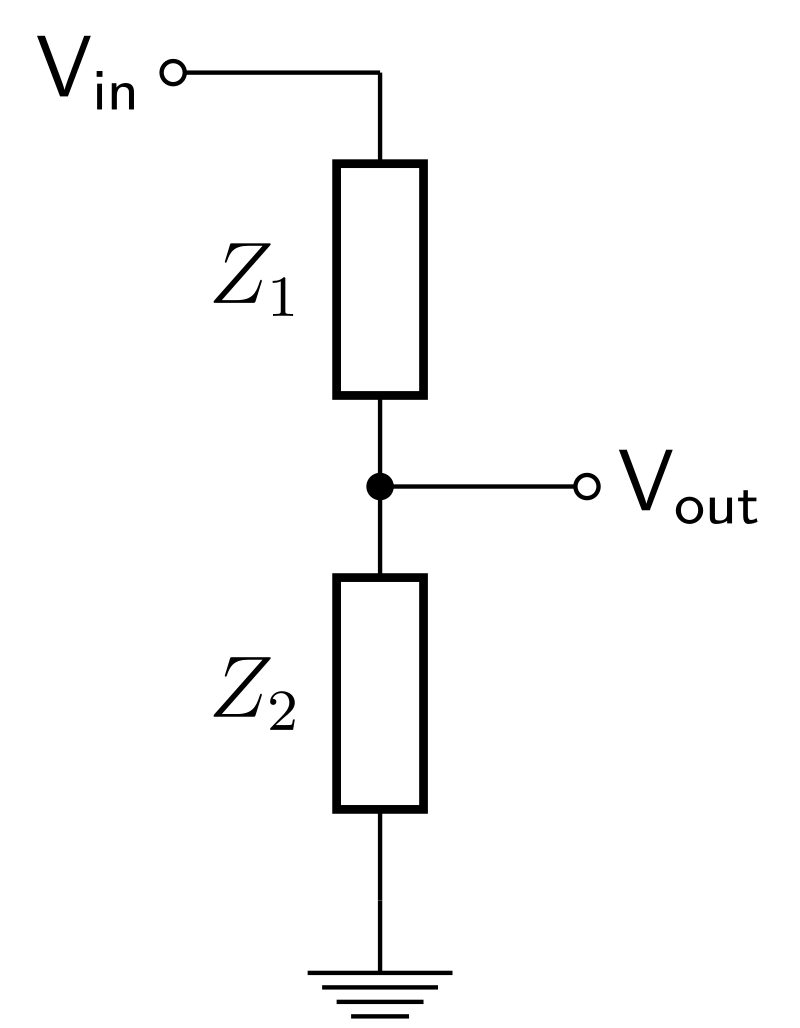
\includegraphics[width=0.2\textwidth]{images/potential divider.png}
    \caption{Potential divider circuit}
    \label{fig:potential-divider-circuit}
\end{figure}

Consider the above circuit where two impedances $Z_1, Z_2$ are connected in series. This circuit is a potential divider, and it is frequently used in all of electronics. 

\begin{proposition}[Potential divider]
    For a potential divider circuit, the voltage across $Z_2$ is:

    \[ V_2 = \frac{Z_2}{Z_1 + Z_2}V_{\text{in}} \]
\end{proposition}

\begin{proof}
    The series grouping of these impedances yields us that $Z_T = Z_1 + Z_2$. Therefore, the total voltage is given by:

    \[ V_{\text{in}} = i(Z_1 + Z_2) \]

    At the same time, the voltage across $Z_2$ is given by $V_2 = iZ_2$. By dividing the two relationships, we obtain:

    \[ \frac{V_{\text{in}}}{V_2} = \frac{Z_1 + Z_2}{Z_2} \]

    Therefore:

    \[ V_2 = \frac{Z_2}{Z_1 + Z_2}V_{\text{in}} \]
\end{proof}

Lastly, Ohm's law and Kirchhoff's laws (which will be discussed at a later point in the course) apply to impedances just as they do for normal resistances. The difference is that both the voltage and the current ($v$ and $i$) now vary with time and can be expressed in terms of complex numbers.

\subsubsection{Capacitors}

We will now analyze the behavior of capacitors. Consider the circuit below. Before the voltage source is connected to the circuit, the capacitor contains no charge. However, at time $t = 0$, the capacitor begins charging. We want to determine the dependency $v = v(t)$ for the voltage across the terminals of a capacitor.

\begin{figure}[h]
    \centering
    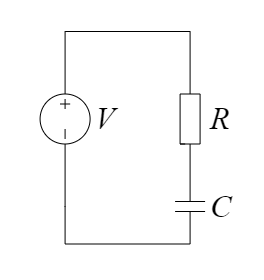
\includegraphics[width=0.2\textwidth]{images/rccircuit.png}
    \caption{R-C Circuit}
    \label{fig:rc-circuit}
\end{figure}

We know that $i = C\frac{dv}{dt}$. Since the two circuit elements are in series, we determine that:

\[ V = v + iR \]

Therefore, the voltage across the terminals of the capacitor is governed by the differential equation:

\[ RC\frac{dv}{dt} + v = V \]

By solving this differential equation, we obtain that the time dependency of the voltage across the terminals of the capacitor is given by:

\[ v(t) = V\left(1 - e^{-\frac{t}{RC}}\right) \]

We can observe that $\lim_{t \to \infty} v(t) = V$, so when the capacitor is fully charged, the voltage across the resistor is $0$. Furthermore, we define a time constant that represents the time at which the capacitor is at $1 - \frac{1}{e}$ of the total voltage:

\[ \tau = RC \]

This is essentially a time delay which we can use to control the time and frequency properties of signals in AC circuits. Furthermore, as previously described, the impedance of a capacitor is given by $Z_C = \frac{1}{j\omega C} = -j \frac{1}{\omega C}$. Therefore, a capacitor shifts a signal by $- \frac{\pi}{2}$. We say that it lags the signal.

\subsubsection{Inductors}

We will now switch our attention to the behavior of inductors. Consider an $R-L$ circuit as below. The inductor initially contains no current. At time $t = 0$, current starts flowing into the inductor. We wish to analyze the dependency $i = i(t)$ at the terminals of the inductor.

\begin{figure}[h]
    \centering
    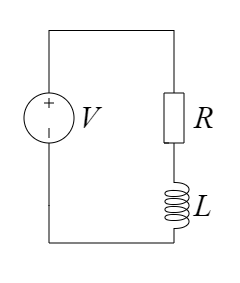
\includegraphics[width=0.2\textwidth]{images/rlcircuit.png}
    \caption{R-L Circuit}
    \label{fig:rl-circuit}
\end{figure}

As previously proved, the voltage across the terminals of a conductor is given by:

\[ v = L\frac{di}{dt} \]

Furthermore, we know that $V = iR + v$. Hence:

\[ L\frac{di}{dt} + iR = V \iff \frac{di}{dt} + \frac{R}{L}i = V \]

This is another first-order ordinary differential equation. By solving it, we obtain that:

\[ i(t) = \frac{V}{R}\left(1 - e^{-\frac{R}{L}t}\right) \]

We observe that just as before, we can define the time constant of an inductor as:

\[ \tau = \frac{L}{R} \]

This time delay allows us, just as before, to control the time and frequency properties of voltages and currents in AC circuits. Furthermore, the impedance of the inductor is $Z_L = j\omega L$, as previously proved. Therefore, there is a phase shift of $\frac{\pi}{2}$ between the signal and the inductor. We say that the inductor leads the signal.

It is also important to note that no inductor or capacitor is perfect, and there will always be ways of representing those imperfections theoretically. For an inductor, this is through a series resistance which represents the resistance of the wire. For capacitors, it is a parallel resistance which represents the leakage current through the dielectric.

\newpage

\subsection{Voltage and current sources. Norton and Thévenin's theorems}

As well as passive components, circuits also require a source of charge in order to function. This can be a battery or a power supply, however, for analysis we utilize either voltage or currents sources. For DC, the arrow always points to the highest potential or more positive side of the source. For AC, it refers to the reference point for all phase measurements relevant to that source.

\subsubsection{Voltage sources}

\begin{definition}[Ideal voltage source]
    An ideal voltage source will always have a constant voltage $V$ (or an amplitude $v$) across its terminals and no resistance, i.e. the resistance between both terminals will always be null.
\end{definition}

We can make an ideal voltage source appear real by placing a resistance $R_S$ in series with it. We say that $R_S$ is the internal resistance of the source. For an AC voltage source, $R_S$ would be replaced by a source impedance $Z_S$.

\subsubsection{Current sources}

The voltage source is a very useful model for a battery or source of charge, however it does not always prove the best means of solving a circuit, especially if it involves current based devices such as transistors, or integrated circuits.

\begin{definition}[Ideal current source]
    An ideal current source will always produce a constant current $I$ (or an amplitude $i$) across its terminals, and have infinite resistance.
\end{definition}

\begin{figure}[h]
    \centering
    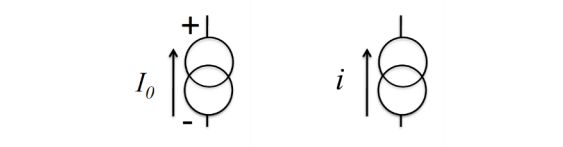
\includegraphics[width=0.75\textwidth]{images/currentsource.png}
    \caption{Representation of current sources}
    \label{fig:current-sources}
\end{figure}

Once again, in order to represent a non-ideal current source, we can place an internal resistance $R_S$ in parallel with the source.

\subsubsection{Norton and Thévenin's theorems}

By means of analysis, we can deduce that a voltage source in series with a resistance $R_S$ is equivalent to a current source in parallel with the same resistance $R_S$, as both charge sources should work in a similar manner. For this reason, we introduce the two following theorems which allows us to greatly simplify any circuit.

\begin{theorem}[Thévenin's theorem]
    Any linear two-terminal network may be replaced by a voltage source $V_{T}$ in series with a resistance $R_{T}$.
\end{theorem}

The Thévenin voltage is equal to the voltage of the open circuit. In order to calculate the Thévenin resistance, we short all the voltage sources and open the current sources, and then calculate the equivalent resistance between the two terminals. Therefore:

\[ V_T = V_{\text{open circuit}} \text{   and   } R_T = \frac{V_{\text{open circuit}}}{I_{\text{short circuit}}} \]


\begin{theorem}[Norton's theorem]
    Any linear two-terminal network may be replaced by a current source $I_N$ in parallel with a resistance $R_N$.
\end{theorem}

The Norton current is equal to the short circuit current, while the Norton resistance is calculated just as the Thévenin resistance. Therefore:

\[ I_N = I_{\text{short circuit}} \text{   and   } R_N = \frac{V_{\text{open circuit}}}{I_{\text{short circuit}}} \]

We can link the two theorems (transformations) by the following set of relationships: $R_T = R_N$, $V_T = I_NR_N$, and $I_N = \frac{V_T}{R_T}$. This technique of replacing one part of a circuit with an equivalent model is known as superposition. Furthermore, this superposition principle can be extended - suppose we have a circuit with sources (either voltage or current sources) $S_1, S_2, \dots, S_n$. Therefore, if we want to determine the voltage (or current) across a certain impedance, we can fix a source $S_i$, $1 \leq i \leq n$ and remove all the others (by shorting the other voltage sources and opening the current sources). By repeating this algorithm for all $i$ between $1$ and $n$, we can add all the individual contributions from each source and determine the total voltage (or current) across the impedance.

\newpage

\subsection{Kirchhoff's laws}

In 1846, Gustav Kirchhoff proposed that in a circuit, the work done by a battery or power source in driving a current around it is equal to the energy dissipated within the circuit. In other words, energy must be conserved.

\subsubsection{Kirchhoff's voltage and current laws}

\begin{proposition}[Kirchhoff's voltage law]
    Consider a closed loop with voltage sources $V_1, V_2, \dots, V_m$ and resistances $R_1, R_2, \dots, R_n$. Therefore, we must have that:

    \[ \sum_{i = 1}^m V_i = \sum_{i = 1}^n R_i \]
\end{proposition}

To see why this is true, we can imagine a closed loop with various voltage sources and resistances. We know that $P = \frac{dW}{dt}$, so for a constant power, it is true that $W = P\Delta t$. By writing the work done as $I_iV_i\Delta t$ and the energy lost as $I_i^2R_i\Delta t$, we can obtain the above result.

This law is the basis for mesh analysis, where the mesh refers to the closed loop. The exact polarities of the currents will often depend on the values of the sources, but the sum must always equal nought.

\begin{proposition}[Kirchhoff's current law]
    Consider a node $N$ in a circuit with currents $I_i, 1 \leq i \leq n$ flowing in and out of the node. Therefore:

    \[ \sum_{i = 1}^n I_i = 0 \]
\end{proposition}

This is true because charge must be conserved, and therefore all charge that goes in the system must be equal to the charge that goes out of the system. To prove this, we note that each wire that goes into the node carries a total current $i = \frac{dq}{dt} \iff dq = idt$. Now, because we do not know which currents go out and in of the node, we can assign a plus sign to those that go out, and a minus sign to those that go in. Therefore, since total charge is conserved:

\[ \sum_{k = 1}^n dq_n = 0 \iff \sum_{k = 1}^n i_kdt = 0 \iff \sum_{k = 1}^n i_k = 0 \]

This law forms the basis for nodal analysis which is one of the most important tools that we have for analysing circuits. It is important to note that the direction of the currents may not be known at the time of the analysis, and therefore it is always a good practice to assume all currents are going into the node.

\begin{example}[Nodal analysis]

    Consider the circuit in the figure below. Suppose we wish to find the voltage across the $2\Omega$ resistor. To do this, we label each node with a letter and then proceed to measure all the voltages across a conventional node (i.e., we choose the ground node). For our example, we can assume $V_c = 0$.

    We can now write the following system of equations:

    \[ \frac{6 - V_b}{8} + \frac{0 - V_b}{2} + \frac{4 - V_b}{4} = 0 \]

    This allows us to find the potential at point $b$ in the circuit. Therefore:

    \[ 6 - V_b - 4V_b + 8 - 2V_b = 0 \]

    This equation is then equivalent to:

    \[ 7V_b = 14 \iff V_b = 2V \]

    Now, we know that the voltage across the $2\Omega$ resistor is simply $V_b - V_c = 2V$. Furthermore, we can easily find the current through the resistor:

    \[ V_b - V_c = IR \iff I = 1A \]
    
    \begin{figure}[h]
    \centering
    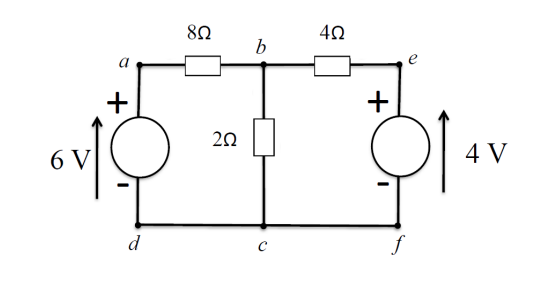
\includegraphics[width=0.6\textwidth]{images/nodal.png}
    \caption{Nodal analysis example}
    \label{fig:nodal-analysis}
    \end{figure}

    This very simple example allows us to understand the power of nodal analysis. Applying Kirchhoff's voltage law would, in fact, require two equations for both loops. We can observe that nodal analysis reduces the number of equations by $1$. However, nodal analysis allows us to first find the potentials, and then the currents. If our goal is to rapidly determine the current passing through a certain impedance, it might be more useful to use Kirchhoff's voltage law and mesh analysis.
\end{example}

\subsubsection{Bridge circuits}

Bridge circuits are used in instrumentation applications when a property such as resistance or impedance is to be measured. They all have the same basic symmetry, with the Wheatstone bridge used for measuring resistance, and the Wein and Maxwell bridges used for impedances. An ammeter connects the two sides of the bridge - at the balance point, there is no current through $(M)$ and the two sides are at the same voltage. We can then derive a useful relationship linking the four impedances in a bridge.

\begin{figure}[h]
    \centering
    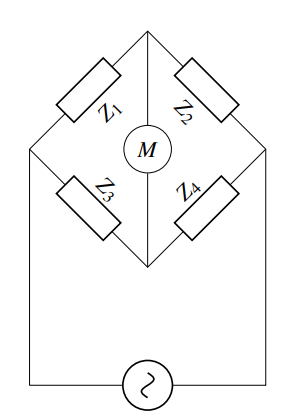
\includegraphics[width=0.2\textwidth]{images/bridge.png}
    \caption{Impedance bridge circuit}
    \label{fig:bridge}
\end{figure}

By applying KVL to the left and right loops, we obtain:

\[ i_1Z_1 = i_2Z_3 \]
\[ i_1Z_2 = i_2Z_4 \]

By dividing the two relationships, we then deduce that in order for the bridge to be balanced, we must have that:

\[ \frac{Z_1}{Z_2} = \frac{Z_3}{Z_4} \iff Z_1Z_4 = Z_2Z_3 \]

We can generally deduce two balance conditions from this equation. In order to do so, we must impose that:

\[ \Im{\left(Z_1Z_4\right)} = \Im{\left(Z_2Z_3\right)} \]
\[ \Re{\left(Z_1Z_4\right)} = \Re{\left(Z_2Z_3\right)} \]

In other words, because the two products are complex numbers, in order for them to be equal, we must have that the real and imaginary parts are mutually equal.

\newpage

\subsection{Analysing AC circuits}

Using the principles of complex impedance, Ohm's law and Kirchhoff's laws, we can now analyse more complicated circuits involving both capacitors and inductors.

\subsubsection{First-order low pass filters}

Passive components like inductors and capacitors can be used to form filters which can control the passage of high and low frequency signals. These are very commonly used in analogue circuits such as audio amplifiers, as well as in digital circuits to reduce the effects of noise interference.

\begin{figure}[h]
    \centering
    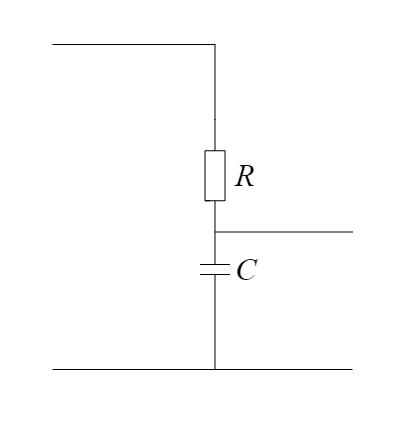
\includegraphics[width=0.3\textwidth]{images/filter1.png}
    \caption{Low-pass filter}
    \label{fig:filter-low}
\end{figure}

Consider the above circuit. We wish to see what happens with the voltage across the capacitor at both DC ($\omega = 0$) and high AC frequencies. Note that $\omega = 2\pi f$, so the relationship between angular frequency and frequency is directly proportional.

The combination of the resistor and the capacitor form a potential divider, hence the voltage across the capacitor is:

\[ v_o = \frac{Z_C}{Z_R + Z_C}v_i = \frac{\frac{1}{j\omega C}}{R + \frac{1}{j\omega C}}v_i \]

The above relationship can be rewritten as:

\[ v_o = \frac{1}{1 + j\omega RC}v_i \]

We observe that when $\omega = 0$, $v_o = v_i$, and as $\omega \to \infty$, $v_o \to 0$. Hence, the above circuit passes low frequency, but blocks high frequencies. This is known as a first-order low pass filter. Moreover, we the gain of this circuit can be expressed as:

\[ \left|\frac{v_o}{v_i}\right| = \frac{1}{\sqrt{1 + (\omega RC)^2}} \]

There is an important transition from the coarse analysis above where the frequency starts to decrease the impedance of the capacitor. We define this point as where the magnitude of the voltage gain is reduced by a factor of $\sqrt{2}$. This is often referred to as the $0.7$, or $70\%$ voltage point. In terms of power, it is referred to as the point where power is reduced by a factor of $2$, or the $3dB$ point. Consider a first-order gain expression of the type:

\[ z = \frac{a + jb}{c + jd} \]

Note that generally, $a$ and $c$ would be real (resistance) values, whereas $b, d$ are frequency dependant impedances. Therefore, the condition where the $|z|$ is reduced by $\sqrt{2}$ is:

\[ d = c \]

Now, we know that the complex gain is expressed as:

\[ \frac{v_o}{v_i} = \frac{1}{1 + j\omega RC} \]

Therefore, by the above theorem, the angular frequency at which the gain is reduced by $\sqrt{2}$ is given by the condition:

\[ \omega_0RC = 1 \iff \omega_0 = \frac{1}{RC} \iff f_0 = \frac{1}{2\pi RC} \]

\begin{definition}[Power gain]
    We define the power gain of a circuit in decibels as:

    \[ G_P = 10\log_{10}\left|\frac{P_o}{P_i}\right| \]
\end{definition}

\begin{definition}[Voltage gain]
    We define the voltage gain of a circuit in decibels as:

    \[ G = 20\log_{10}\left|\frac{v_o}{v_i}\right| \]
\end{definition}

\subsubsection{First-order high pass filter}

Consider the $R-C$ circuit shown below. Note that it is similar to the previously analyzed low pass filter, however the positioning of the resistor and capacitor is changed.

\begin{figure}[h]
    \centering
    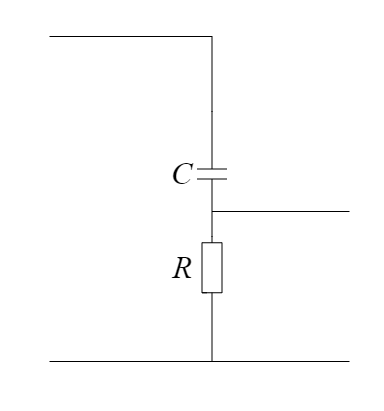
\includegraphics[width=0.3\textwidth]{images/filter2.png}
    \caption{High pass filter}
    \label{fig:filter-high}
\end{figure}

Proceeding in a similar manner, the voltage across the resistor is:

\[ v_o = \frac{R}{R + \frac{1}{j\omega C}}v_i \iff \frac{v_o}{v_i} = \frac{j\omega RC}{1 + j\omega RC} \]

We can observe that for $\omega = 0$, $v_o = 0$, and as $\omega \to \infty$, $v_o \to v_i$. Therefore, this circuit blocks low frequency and passes high frequencies. This is known as a first-order high pass filter. Moreover, the $3dB$ point can be obtained using the same algorithm as before:

\[ 1 = \omega_0RC \iff f_0 = \frac{1}{2\pi RC} \]

This type of circuit is often used in audio circuits to cut off DC voltages and frequencies below $20$ Hz.

One of the limitations of such first-order filters is that the slope of the stop band is limited to $20$ dB per decade ($20$ dB increase for a $10$x increase in frequency and vice-versa), and many applications require a much higher cutoff slope. Higher order filters can achieve this, but often at the expense of complexity or stability.

\newpage

\subsection{Resonant circuits}

\begin{proposition}[Series RLC circuit]
We are now considering the case of resonance, i.e. when the system oscillates with its natural frequency. Consider a series RLC circuit. We wish to find what happens when the reactive elements cancel each other out.

The impedance of this circuit is simply given by:

\[ Z = R + j(\omega L - \frac{1}{\omega C}) \]

At resonance, the reactivbe components cancel out their impedance, meaning that the imaginary term above vanishes. Hence, for resonance, we must always set the condition $\Im(Z) = 0$. Therefore:

\[ \omega L = \frac{1}{\omega C} \iff \omega^2 = \frac{1}{LC} \]

Therefore, the angular frequency at resonance is given by $\omega = \frac{1}{\sqrt{LC}}$. If we use the fact that $f = \frac{\omega}{2\pi}$, we obtain:

\[ f = \frac{1}{2\pi\sqrt{LC}} \]

\end{proposition}

\begin{figure}[h]
    \centering
    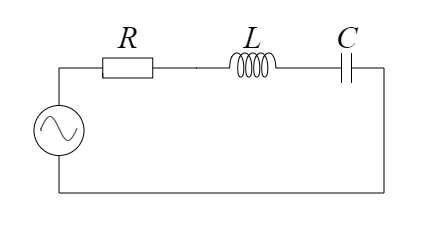
\includegraphics[width=0.5\textwidth]{images/rlc.png}
    \caption{RLC series circuit}
    \label{fig:rlc-series}
\end{figure}

\begin{proposition}[Parallel RLC circuit]
    Consider a parallel RLC circuit. We wish the proceed just as in the previous example in order to determine the resonance condition for a parallel RLC circuit.

    Again, we can determine the complex impedance of the above circuit:

    \[ \frac{1}{Z} = \frac{1}{R} + \frac{1}{j\omega L} + j\omega C = \frac{1}{R} + j(\omega C - \frac{1}{\omega L}) \]

    Therefore, we obtain $\omega C = \frac{1}{\omega L} \iff \omega = \frac{1}{\sqrt{LC}}$. Hence, the condition for a parallel circuit is equivalent to the condition for a series circuit, i.e.:

    \[ f = \frac{1}{2\pi\sqrt{LC}} \]
\end{proposition}

\begin{figure}[h]
    \centering
    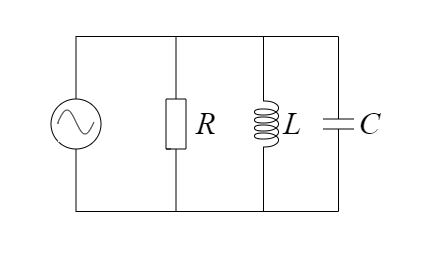
\includegraphics[width=0.45\textwidth]{images/rlcpar.png}
    \caption{RLC parallel circuit}
    \label{fig:rlc-parallel}
\end{figure}

\subsubsection{Q-factor and bandwidth}

The reason circuits are designed to resonate is to be able to have them react to different signal frequencies. This is useful for designing tuning circuits, analogue filters, and so on. The $Q$-factor is a dimensionless design parameter that characterises how underdamped an oscillating system is. In general, the $Q$-factor is defined as the ratio of the energy stored in the system and the energy lost over a cycle. In general:

\[ Q = \omega\frac{M}{\zeta} \]

Where $M$ is the mass, $\omega$ is the angular frequency, and $\zeta$ is the frictional force (in the case of a pendulum). Now, in a circuit the energy stored resides within the inductor and the capacitor, whereas the energy lost is in the resistance, which is dissipated as heat. The energy stored in the capacitor is $\frac{1}{2}CV^2$, and the energy stored in the inductor is $\frac{1}{2}LI^2$.

\begin{proposition}[Q-factor for a series RLC circuit]
    Consider a series RLC circuit. Therefore, the current flowing through each component is identical. Since the $Q$-factor is the energy stored over energy lost, we obtain:

    \[ Q = \omega_0\frac{\frac{1}{2}LI^2}{I_{\text{rms}}^2R} \]

    Since $I_{\text{rms}} = \frac{1}{\sqrt{2}}I$, therefore:

    \[ Q = \frac{\omega_0L}{R} = \frac{X_L}{R} \]

    Equivalently, the $Q$-factor is equal to:

    \[ Q = \frac{1}{\omega_0RC} = \frac{X_C}{R} \]
\end{proposition}

\begin{proposition}[Q-factor for a parallel RLC circuit]
    Consider a parallel RLC circuit. Therefore, since this time the voltage across each component must be equal, it is useful to express the $Q$-factor in terms of the capacitance:

    \[ Q = \omega_0RC = \frac{R}{X_C} \]

    Equivalently, in terms of the inductor:

    \[ Q = \frac{R}{\omega_0L} = \frac{R}{X_L} \]
\end{proposition}

Note that for both cases, the angular frequency is defined as $\omega_0 = \frac{1}{\sqrt{LC}}$, i.e. the angular frequency at resonance.

\begin{definition}[Bandwidth]
    The bandwidth $\Delta f$ is defined as the length of the interval between the two frequencies $f_1$ and $f_2$ where the power output exceeds $50\%$ of the maximum value, i.e.:

    \[ \Delta f = |f_2 - f_1| \]

    This is also known as the full width at half maximum (FWHM).
\end{definition}

\begin{proposition}[Bandwidth equivalence]
    An alternative useful definition (approximation) of the bandwidth, that we normally use in problems is:

    \[ Q = \frac{f_0}{\Delta f} = \frac{\omega_0}{\Delta \omega} \]
\end{proposition}

\begin{proposition}[Series to parallel resistance switch]
    Consider a circuit where we might have an inductor in series with a resistance $R$. We wish to find $R_L$ so that we can change the resistance from being in series to parallel (or vice-versa). As the $Q$-factor must be the same for both the series and parallel inductor:

    \[ Q = \frac{\omega_0L}{R} = \frac{R_L}{\omega_0L} \]

    Likewise, this can be done for a capacitor:

    \[ Q = \frac{1}{\omega_0RC} = \omega_0R_CC \]
\end{proposition}

This proposition then allows us to compute the $Q$-factor of an entire circuit. We first must switch all components to either parallel or series (depending on how the inductor and capacitor are placed), and then compute the total equivalent resistance (either in parallel or series). Then, we simply use $R_T$ in the $Q$-factor definition to determine the total $Q$-factor of a circuit.

\newpage

\subsection{The amplifier model}

A lot of generic circuits can be expressed using a simple two port model with various internal parameters that express the operation of the circuit within. This often lets us to greatly simplify a complicated circuit into a much simpler model that can then be combined with other models to further simplify our work - we have already seen this with the Thévenin and Norton equivalents. The amplifier model usually has three distinct parameters:

\begin{enumerate}
    \item The input impedance (usually a resistance) - $R_{\text{in}}$
    \item The voltage gain - $A$
    \item Output impedance (usually a resistance) - $R_{\text{out}}$
\end{enumerate}

It is also important to note that this model applies only to amplifiers that have linear gain, although it is possible to have an amplifier with a gain that is a function of frequency.

\begin{figure}[h]
    \centering
    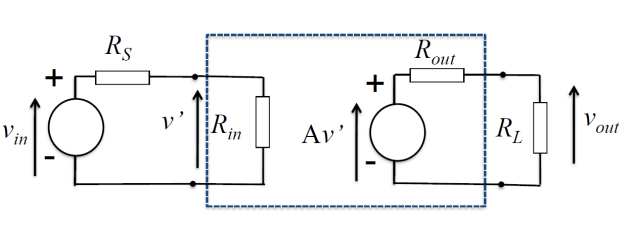
\includegraphics[width=0.75\textwidth]{images/amplifier1.png}
    \caption{Two-port amplifier circuit}
    \label{fig:amplifier}
\end{figure}

Consider the above amplifier circuit. We wish to determine the voltage $v_{\text{out}}$ in terms of $v_{\text{in}}$. Therefore:

\[ v' = \frac{R_{\text{in}}}{R_S + R_{\text{in}}}v_{\text{in}} \]

Furthermore:

\[ v_{\text{out}} = \frac{R_L}{R_{\text{out}} + R_L}Av' \]

By combining the two relationships, we therefore obtain:

\[ v_{\text{out}} = \frac{AR_LR_{\text{in}}}{(R_S + R_{\text{in}})(R_{\text{out}} + R_L)}v_{\text{in}} \]

This is also known as the voltage gain of the amplifier. Moreover, we can cascade amplifiers to obtain even a higher gain - the analysis stays the same, and we can also express the result of an amplifier in terms of current gain. Just as before, we can use a decibel scale to express the power gain of an amplifier, which is defined as:

\[ G_P = 10\log_{10}\left(\frac{P_{\text{out}}}{P_{\text{in}}}\right) \]

Where the output power is the power across the load resistance $R_L$ and the input power is the power across the input resistance $R_{\text{in}}$.

\begin{proposition}[Maximum power transfer theorem]
    Consider a power amplifier that drives a load $R_L$. If we have an amplifier with an output resistance $R_{\text{out}}$, in order to maximize the power gain, we must have $R_L = R_{\text{out}}$.
\end{proposition}

\begin{proof}
    The output voltage is $v_{\text{out}} = \frac{R_L}{R_L + R_{\text{out}}}Av'$. Since the power dissipated in that resistance is $P = \frac{v_{\text{out}}^2}{R_L}$, we deduce that:

    \[ P = \frac{A^2v'^2R_L}{(R_L + R_{\text{out}})^2} \]

    For maximum power, we must impose that $\frac{dP}{dR_L} = 0$. Hence:

    \[ A^2v'^2 \frac{(R_L + R_{\text{out}})^2 - 2R_L(R_L + R_{\text{out}})}{(R_L + R_{\text{out}})^4} = 0 \]

    Since $R_L > 0$, the solution to the above equation is:

    \[ R_L = R_{\text{out}} \]

    Therefore, when the load resistance is equal to the output resistance, the power gain is maximized.
\end{proof}

Another important aspect of an amplifier is its frequency response, as the gain may be a function of frequency and there may be reactive elements at the input and output ports. Consider the following circuit:

\begin{figure}[h]
    \centering
    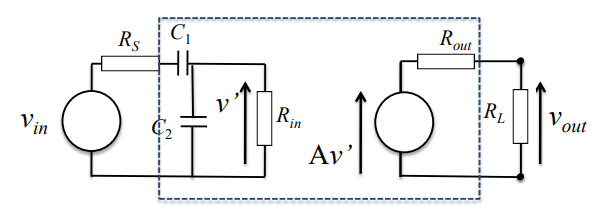
\includegraphics[width=0.75\textwidth]{images/amplifier2.png}
    \caption{Frequency-dependent amplifier}
    \label{fig:amplifier2}
\end{figure}

We now analyze this amplifier for both low and high frequencies. At low frequencies, $C_2$ becomes an open circuit, and at high frequencies, $C_1$ becomes a short circuit. Therefore, $C_1$ dominates at low frequencies and $C_2$ dominates at high frequencies. Therefore, for low frequencies:

\[ v_{\text{out}} = \frac{AR_L}{R_L + R_{\text{out}}}v' \]
\[ v' = \frac{R_{\text{in}}}{R_{\text{in}} + R_S + \frac{1}{j\omega C_1}}v_{\text{in}} = \frac{j\omega C_1R_{\text{in}}}{1 + j\omega C_1(R_{\text{in}} + R_S)}v_{\text{in}} \]

The $3$ dB point is attained by this amplifier for $1 = \omega C_1(R_{\text{in}} + R_S)$. Therefore, the first frequency is:

\[ f_1 = \frac{1}{2\pi C_1(R_{\text{in}} + R_S)} \]

Now, at high frequencies, $C_1$ becomes a short circuit. The parallel impedance of $C_2$ and $R_{\text{in}}$ is:

\[ Z = \frac{\frac{1}{j\omega C_2} R_{\text{in}}}{R_{\text{in}} + \frac{1}{j\omega C_2}} = \frac{R_{\text{in}}}{1 + j\omega C_2R_{\text{in}}}\]

Therefore, the voltage $v'$ can be expressed as:

\[ v' = \frac{\frac{R_{\text{in}}}{1 + j\omega C_2R_{\text{in}}}}{R_S + \frac{R_{\text{in}}}{1 + j\omega C_2R_{\text{in}}}}v_{\text{in}} = \frac{R_{\text{in}}}{R_{\text{in}} + R_S + j\omega C_2R_{\text{in}}R_S}v_{\text{in}} \]

Therefore, the $3$ dB condition is given by:

\[ R_S + R_{\text{in}} = \omega C_2R_{\text{in}}R_S \iff \omega = \frac{R_S + R_{\text{in}}}{C_2R_{\text{in}}R_S} \]

And hence, the second cutoff frequency is:

\[ f_2 = \frac{R_S + R_{\text{in}}}{2\pi C_2R_{\text{in}}R_S} \]

And we can obtain the midband $\Delta f = |f_2 - f_1|.$

\newpage

\subsection{Diodes}

Up until now, we have only looked at insulating and conducting materials. The main factor determining how strongly bound the electrons are is the atomic structure of the material, i.e. the arrangement of the atoms. An example of this is Carbon - diamond is an excellent insulator, whereas graphite is a reasonably good conductor - the only difference between these two materials is the arrangement of the atoms. From conductors, we can make resistors, capacitors and inductors. However, they suffer from the issue that they are linear, and their properties cannot be easily controlled - mainly because there are so many free electrons. However, if we could find a type of material where the electron density was low and could be controlled, we could make a wide range of devices - these materials are called semiconductors. Note that insulators (dielectrics) have fixed charges, whilst conductors (such as metals) have lots of free charges.

Silicon is the most common material in use in today's electronic devices. At low temperatures, Silicon is an insulator, and as the temperature is increased, it becomes conducting. Therefore, it is called a semiconductor. 

Additionally, its properties may be dramatically altered by the incorporation of dopant atoms in the crystal. To add extra electrons, we dope with a pentavalent metal (Phosphorous, Antimony or Arsenic), and to add extra holes, we dope with trivalent metals (Boron, Gallium or Indium). If we add a pentavalent dopant atom, we end up with the situation that one of the five valence electrons is freed and we describe the material as $n$-type (negative charge carriers). A similar situation is true for trivalent dopants as holes are positively charged - the material is said to be $p$-type.

At the heart of semiconductor technology is the $p-n$ junction. This is a structure where the doping abruptly changes from $p$-type to $n$-type. It can be made from doping a crystal from both ends. This results in a region where there are no free electrons or holes, which is known as the depletion region. This then produces an electric field which opposes diffusion.

If the junction is reversed biased (more positive potential of the voltage source connected to the $n$-type), we obtain a reverse saturation current $I_0$ on the order of nanoamps. Conversely, if the polarity is reversed, the junction is said to be forward biased - we obtain a diffusion current on the order of milliamps.

This characteristic of the $p-n$ junction of allowing significantly more current to flow in one direction than the other is known as rectification, and this device is commonly known as a $\textbf{diode}$.

\begin{figure}[h]
    \centering
    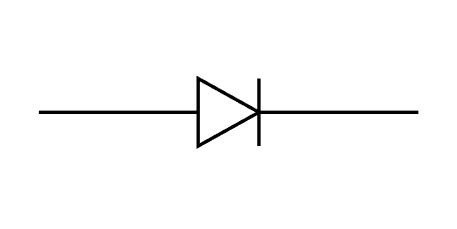
\includegraphics[width=0.75\textwidth]{images/diode1.png}
    \caption{Diode}
    \label{fig:diode1}
\end{figure}

The forward bias relationship between $I$ and $V$ for a diode (the diode's characteristic) is given by:

\[ I \approx I_0\left(e^{\frac{e\eta V}{k_BT}} - 1\right) \]

This is a non-linear function, and in order to solve problems involving diodes, we must always look at the $I-V$ characteristic of the diode and determine its operating point. Consider the following circuit involving a voltage source $V$, a resistor $R$, and a diode.

\begin{figure}[h]
    \centering
    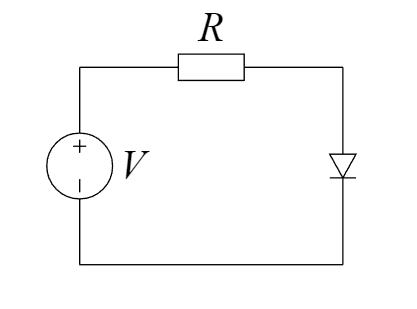
\includegraphics[width=0.5\textwidth]{images/diode2.png}
    \caption{Diode circuit example \#1}
    \label{fig:diode2}
\end{figure}

Because in the above circuit, the current flows in the same direction as the way the diode is pointing, we deduce that:

\[ V = IR + V_D \iff I = \frac{V - V_D}{R} \]

Therefore, we have obtained a linear function that describes the current passing through the diode as a function of the voltage. Now, we can intersect the $I-V$ characteristic of the diode with this function and deduce its operating parameters:

\begin{figure}[h]
    \centering
    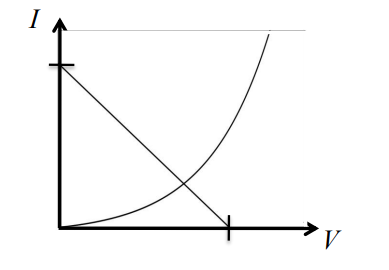
\includegraphics[width = 0.5\textwidth]{images/diode3.png}
    \caption{Intersection of diode characteristic with linear function}
    \label{fig:diode3}
\end{figure}

The intersection between these two curves then gives us the operating point of the diode in our specific circuit. We can then use this point $(V, I)$ to further solve for everything in the circuit. We will now move forward to a more complicated circuit and deduce how to compute the load line in more complex cases.

\newpage

\begin{figure}[h]
    \centering
    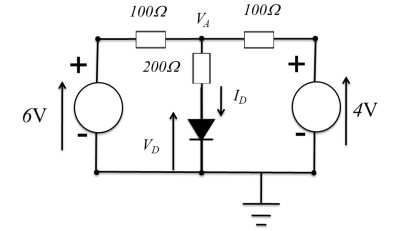
\includegraphics[width = 0.5\textwidth]{images/diode4.png}
    \caption{Circuit involving a diode}
    \label{fig:diode-circuit}
\end{figure}

We will assign $V_D$ to be the voltage across the diode. By means of nodal analysis, we obtain:

\[ \frac{6 - V_A}{100} + \frac{V_D - V_A}{200} + \frac{4 - V_A}{100} = 0 \]

Furthermore, the current across the diode is:

\[ I_D = \frac{V_A - V_D}{200} \]

We can now eliminate $V_A$ by using $V_A = 200I_D + V_D$ to obtain:

\[ I_D = \frac{1}{50} - \frac{1}{250}V_D \]

\newpage

\subsection{Field effect transistors (FETs)}

The semiconducting properties of silicon can also be controlled by either an external action - an electric field or an applied current. If the doping levels are controlled correctly, then it is possible to create a large current flow with a much smaller input and create various forms of gain. In the continuation of this course, we will analyze metal oxide semiconductor field effect transistors (MOSFETs).

There are different types of MOSFETs:

\begin{enumerate}
    \item $n$-channel enhancement \& $n$-channel depletion
    \item $p$-channel enhancement \& $p$-channel depletion
\end{enumerate}

\begin{figure}[h]
    \centering
    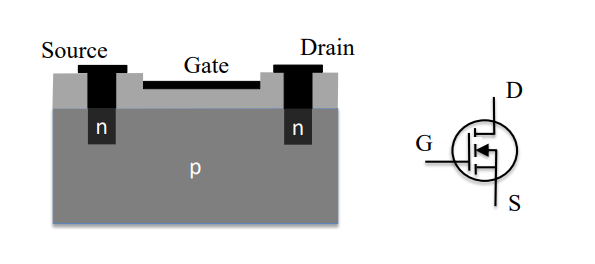
\includegraphics[width = 0.5\textwidth]{images/fet1.png}
    \caption{The n-channel enhancement mode MOSFET}
    \label{fig:fet1}
\end{figure}

If a voltage is applied between the drain (D) and the source (S) when there is no gate voltage, then no drain current will flow, as one of the $p-n$ junctions will always be reverse biased. If a positive gate voltage is now applied, there will be an electric field between the gate and the bottom of the devices, attracting electrons to the interface between the gate oxide and the $p$-type substrate. This is true if:

\[ V_{GS} > V_T \]

Where $V_{GS}$ is the gate-source voltage, and $V_T$ is the threshold value. If we now apply a voltage between the drain and the source $V_{DS}$ as shown above, a current $I_D$ will flow through this inversion layer. For small values of $V_{DS}$, $I_D$ increases linearly and rapidly - this is known as the Ohmic region. As $V_{DS}$ is increased, the difference in voltage between the gate and drain increases, reducing the number of electrons in the inversion layer near the drain, resulting in a levelling off of the $I_D - V_{DS}$ curve. This is known as the saturation region.

\begin{figure}[h]
    \centering
    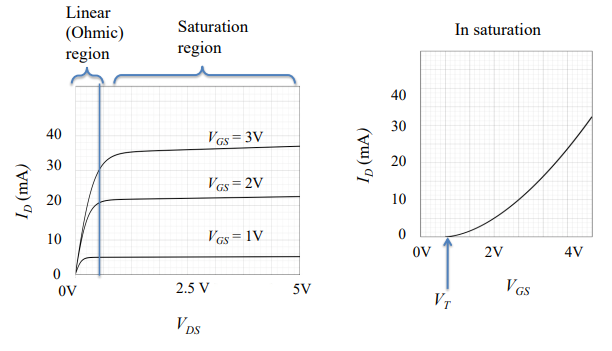
\includegraphics[width = 0.55\textwidth]{images/fet2.png}
    \caption{Transistor graph}
    \label{fig:fet2}
\end{figure}

The difference between an enhancement-mode and depletion-mode MOSFET is that the latter has a built-in $n$-type channel (or $p$-type). The application of a positive gate voltage has the same effect as before, but a negative voltage repels charge away from the channel decreasing the conductivity. The conduction of the channel is controlled by positive and negative $V_{GS}$ which is better suited for bipolar signals (such as AC circuits).

\begin{figure}[h]
    \centering
    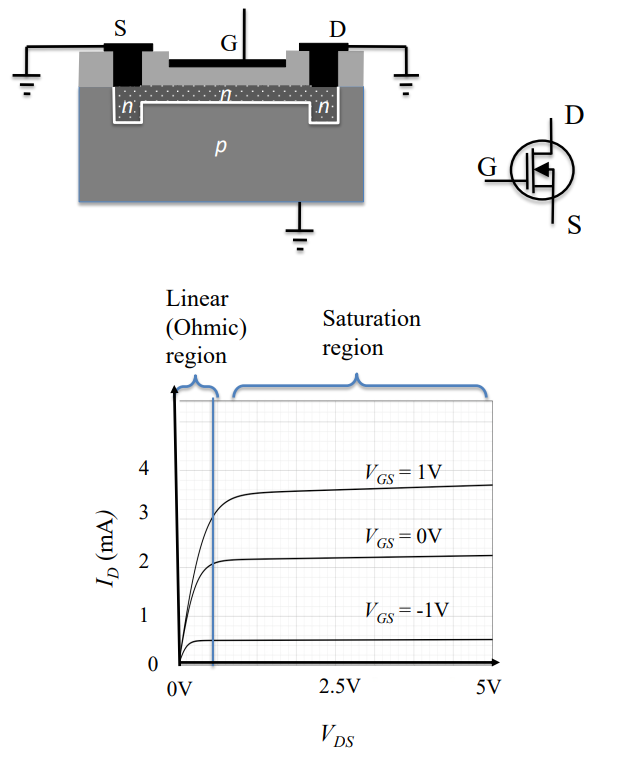
\includegraphics[width = 0.5\textwidth]{images/fet3.png}
    \caption{The n-channel depletion mode MOSFET}
    \label{fig:enter-label}
\end{figure}

Using these characteristics it is now possible to design MOSFET-based circuits, such as amplifiers. There are two stages to designing any FET circuit:

\begin{enumerate}
    \item DC analysis (often called biasing, quiescent setup or operating point)
    \item AC analysis (often called the small signal model)
\end{enumerate}

\subsubsection{The common source amplifier}

The circuit below is known as the common source amplifier, as the source $(S)$ is grounded. The circuit is powered by a DC power source (or battery), $V_{DD}$, which is assumed to be constant with no impedance. The FET can be either ehancement or depletion mode, and this will affect the polarity of $V_G$. The resistor $R_G$ is included, as the source $V_G$ has a very low impedance, and so $R_G$ will set the input impedance of the circuit. Ideally, it should be large (on the order of megaohms).

\newpage

\begin{figure}[h]
    \centering
    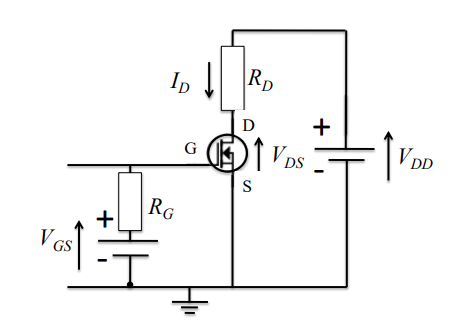
\includegraphics[width = 0.5\textwidth]{images/fet4.png}
    \caption{The common source amplifier}
    \label{fig:enter-label}
\end{figure}

Since $(S)$ is grounded, we know that $V_S = 0 \iff V_{DS} = V_D$. From Kirchhoff's law:

\[ V_{DD} - V_D = I_DR_D \iff V_{DD} - V_{DS} = I_DR_D \]

Therefore, we obtain the loadline of the circuit as:

\[ I_D = \frac{V_{DD} - V_{DS}}{R_D} \]

Note that it is common to set $V_{DS} = \frac{V_{DD}}{2}$ for maximum voltage swing at the output. Using the load line above, we can intersect the MOSFET characteristic to obtain the operating point $V_{GS}$. The FET characteristic also sets the safe operating region (or forbidden zones) for the circuit, based on the following limiting factors:

\begin{enumerate}
    \item non-linear, low-resistance region
    \item maximum limit of $V_{GS}$
    \item maximum power dissipation limit $(V_{DS}I_D)_{\text{max}}$
    \item maximum value of $V_{DS}$
\end{enumerate}

\begin{figure}[h]
    \centering
    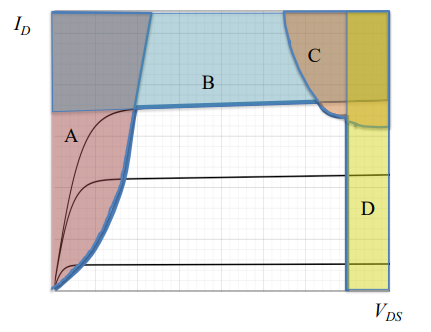
\includegraphics[width = 0.35\textwidth]{images/fet5.png}
    \caption{Safe region for a MOSFET}
    \label{fig:fet5}
\end{figure}

Ideally, the load line should cross diagonally through the safe operating region and the operating point should be as central as possible.

\subsubsection{The self-biased MOSFET amplifier}

The main problem of the common source amplifier circuit is the need for $V_G$ - practical depletion mode MOSFET amplifier circuits use the self-biased amplifier, where $V_{GS} < 0$.

\begin{figure}[h]
    \centering
    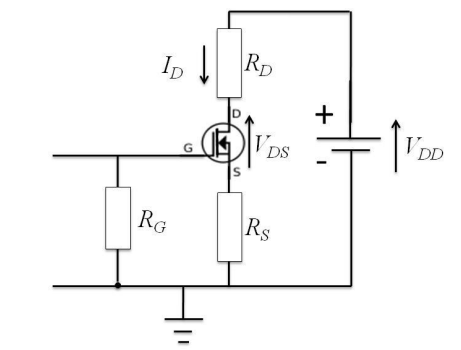
\includegraphics[width = 0.5\textwidth]{images/fet6.png}
    \caption{Self-biased MOSFET amplifier}
    \label{fig:enter-label}
\end{figure}

In the above amplifier circuit, we require that $R_G \to \infty$ so that the gate is held at ground potential. In practice, we utilize values of $R_G \approx M\Omega$. Because of this, the gate current is null. Hence:

\[ V_{GS} = V_G - V_S = -V_S \iff V_S = -V_{GS} \]

Therefore:

\[ V_S - 0 = I_DR_S \iff I_DR_S = -V_{GS} \iff R_S = -\frac{V_{GS}}{I_D} \]

We can also determine the resistance $R_D$ so that the amplifier works at the given operating point. We first need to determine the potential of the drain:

\[ V_{DS} = V_D - V_S \iff V_D = V_{DS} + V_S \iff V_D = V_{DS} - V_{GS} \]

By applying Kirchhoff's law again, we obtain:

\[ V_{DD} - V_D = I_DR_D \iff R_D = \frac{V_{DD} - V_D}{I_D} \]

\begin{proposition}[Maximum voltage swing condition]
    For any MOSFET circuit, in order to obtain the maximum voltage swing at the output, we must set:

    \[ V_{DS} = \frac{1}{2}V_{DD} \]
\end{proposition}

It is also quite common to see self-biased circuits designed for enhancement mode MOSFETs where $V_{GS} > 0$ to set a suitable operating point. In this case, the gate voltage is set by the two resistances $R_1, R_2$, forming a potential divider. Therefore, $V_{GS}$ is set by the difference between the gate and the source potential. Note that the parallel combination of $R_1$ and $R_2$ now sets the input impedance of the amplifier.

\newpage

\begin{figure}[h]
    \centering
    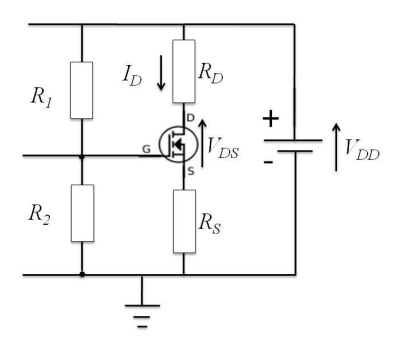
\includegraphics[width = 0.5\textwidth]{images/fet7.png}
    \caption{Potential divider self-biased MOSFET amplifier}
    \label{fig:enter-label}
\end{figure}

The voltage across $R_2$ is $V_G$. Therefore:

\[ V_G = \frac{R_2}{R_1 + R_2}V_{DD} \]

Now, since $V_{GS} = V_G - V_S \iff V_S = V_G - V_{GS}$. Therefore, we can determine $R_S$ from:

\[ V_S = I_DR_S \iff R_S = \frac{V_S}{I_D} \]

Now, just as before, $V_{DS} = V_D - V_S \iff V_D = V_{DS} + V_S$. Hence:

\[ V_{DD} - V_D = I_DR_D \iff R_D = \frac{V_{DD} - V_D}{I_D} \]

Lastly, we can determine both $R_1$ and $R_2$ from the first equation if we know either one of them, or any type of further information. If we do not know anything about the two resistors, we can simply set $R_2 = 1M\Omega$ and determine $R_2$.

\newpage

\subsection{The small signal model (SSM)}

As we have now looked into how to setup the biasing (quiescent) point for a MOSFET, we are now interested in further analyzing such circuits' properties. To do so, we will consider what happens when the operating point becomes slightly shifted, i.e. when a small AC signal is going to be applied at the input.

We know that any change in $I_D$ is due to either a change in $V_{DS}$ or $V_{GS}$, as those can be the only parameters that influence the drain current. By considering the $I_D = I_D(V_{DS})$ characteristic we discussed prior, one can deduce that by keeping $V_{DS}$ constant and by changing $V_{GS}$, we obtain:

\[ \Delta I_D \approx \frac{\partial I_D}{\partial V_{GS}} \Delta V_{GS} \]

Now, by changing $V_{DS}$ and keeping $V_{GS}$ constant, we obtain:

\[ \Delta I_D \approx \frac{\partial I_D}{\partial V_{DS}} \Delta V_{DS} \]

By summing the two contributions together, the approximate change in $I_D$ due to a shift in both voltages is equal to:

\[ \Delta I_D = \frac{\partial I_D}{\partial V_{DS}}\Delta V_{DS} + \frac{\partial I_D}{\partial V_{GS}} \Delta V_{GS} \]

Since the shift in both waveforms is due to an AC signal, we will define the following new quantities:

\begin{enumerate}
    \item $i_d = \Delta I_D$, the drain current
    \item $v_{gs} = \Delta V_{GS}$, the gate-source voltage
    \item $v_{ds} = \Delta V_{DS}$, the drain-source voltage
    \item $g_m = \frac{\partial I_D}{\partial V_{GS}}$, the mutual conductance
    \item $\frac{1}{r_d} = \frac{\partial I_D}{\partial V_{DS}}$, the drain resistance
\end{enumerate}

By using this newly established notation, we can now obtain the small signal model equation.

\begin{proposition}[The small signal model equation]
    Any biased DC FET circuit can be represented in the small signal model equivalent as:

    \[ i_d = \frac{v_{ds}}{r_d} + g_mv_{gs} \]

    Note that this equation simply degenerates into Kirchhoff's current law, i.e. the equation above implies a node into which the drain current comes in, and two currents come out.
\end{proposition}

\begin{figure}[h]
    \centering
    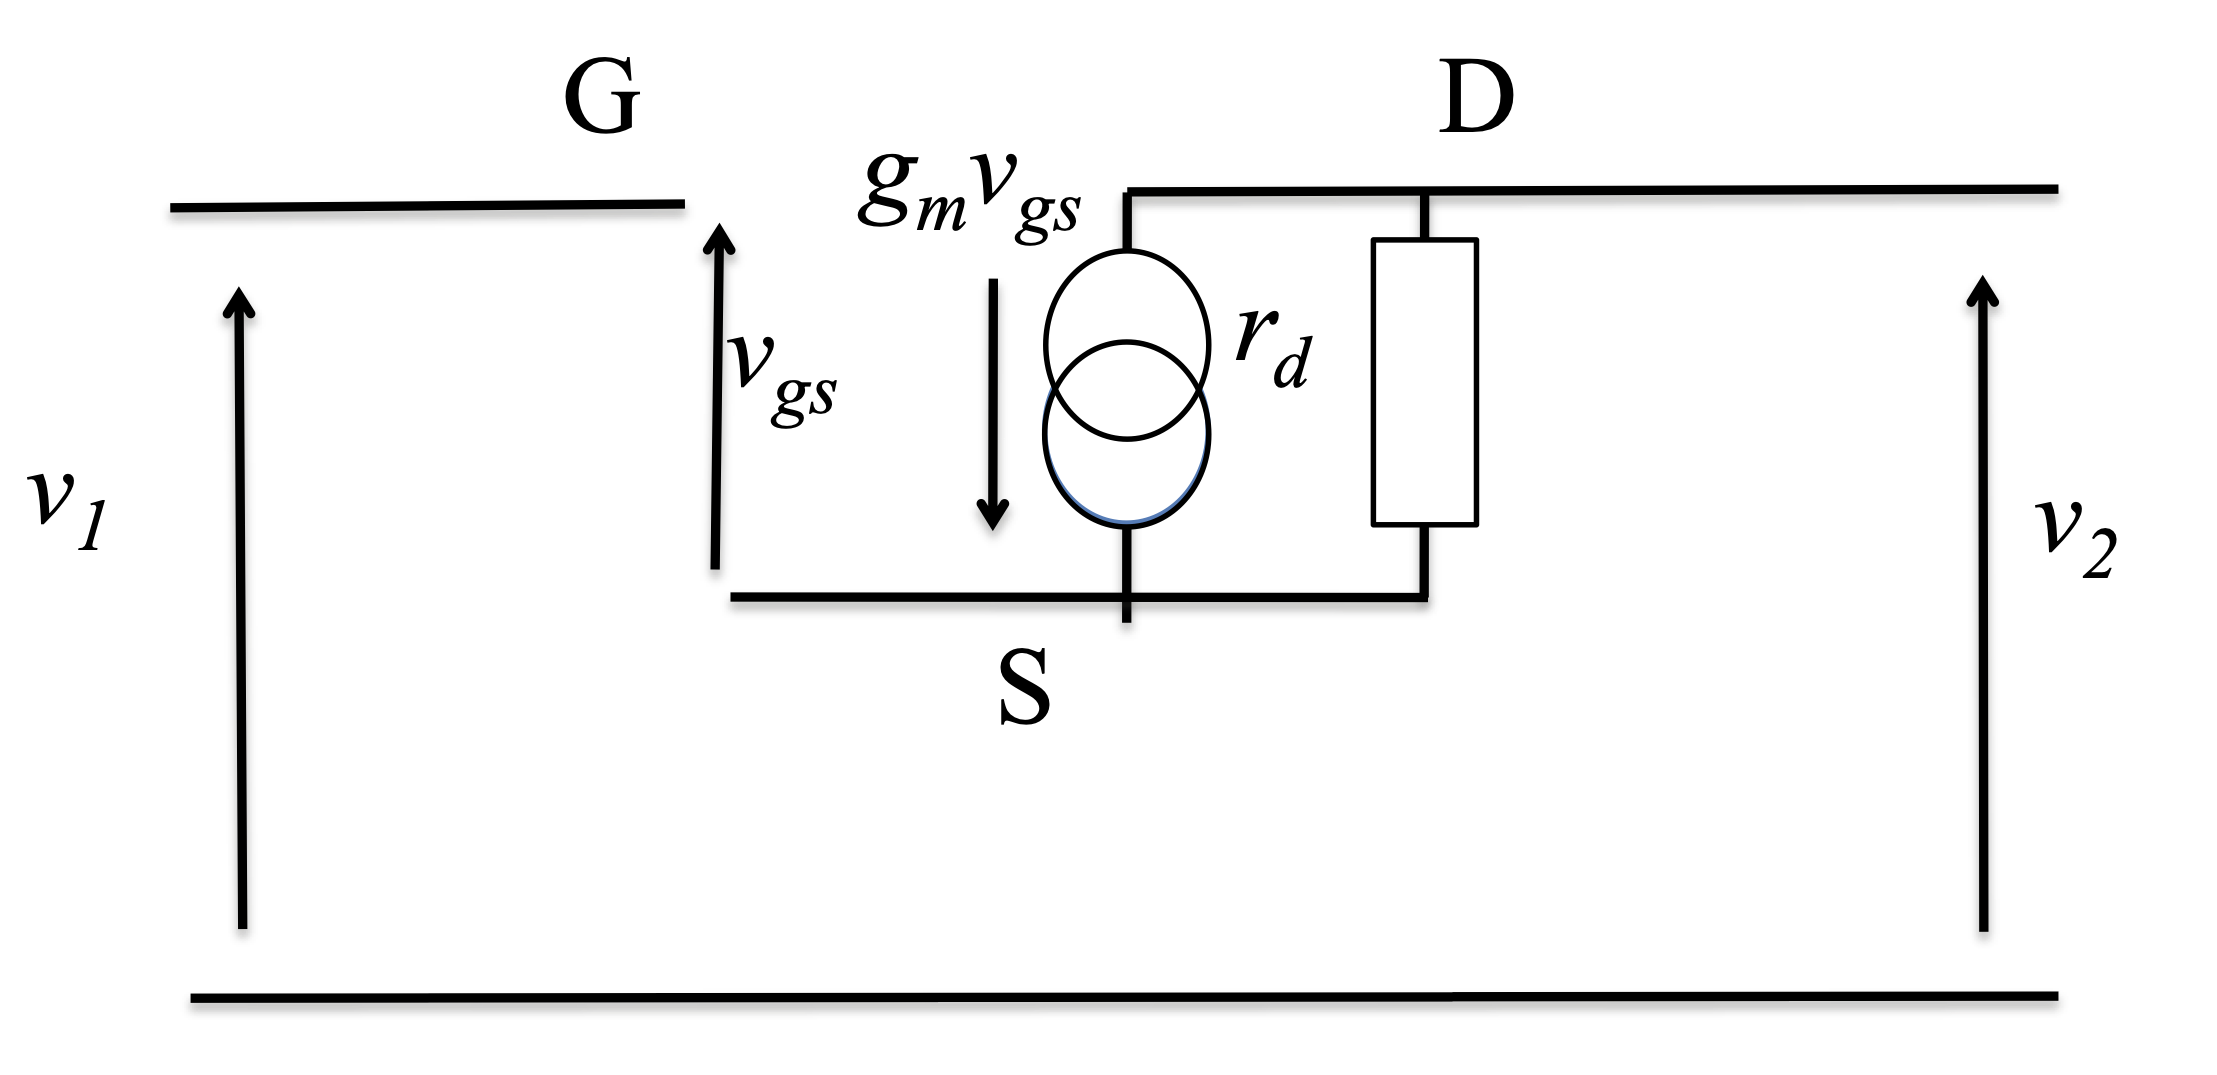
\includegraphics[width = 0.4\textwidth]{images/ssm1.png}
    \caption{The small signal model equivalent circuit}
    \label{fig:ssm-1}
\end{figure}

When transforming a DC FET circuit into its small signal model equivalent, we always starts by drawing the gate, source, and drain, with the aforementioned parameters as in the drawing above. Any ideal voltage source we add is simply represented as a short-circuit, because they do not have any resistance. Note that the line on the bottom is the ground. After that has been done, we can simply add all other circuit elements to their initial position.

Then, we can calculate the input resistance, which should be straightforward, and the output resistance. To compute the output resistance, we proceed as for amplifiers - we always short the input, and determine the resistance at the output following our short (as some components might be shorted due to this).

Furthermore, if we are interested in calculating the input resistance, this is always going to be equal to the grouping of impedances/resistors between the gate and the ground. If we want to calculate the gain, we need to use:

\[ v_\text{in} = v_\text{gs} + v_s \]

Then, we need to use nodal at either (or both) $D$ and $S$. Lastly, if we are interested in finding the output resistance, we must short the input (let $v_\text{gs} = 0$), and apply a voltage $v_x$ and a current $i_x$ to the output.

\newpage

\section{A.C. Power and Transformers}

In this section, we will cover the mini-series of lectures covering power in A.C. circuits and transformers respectively.

\subsection{A.C. Power}

Let us consider the case where we have a voltage source with r.m.s. value $V$ that induces an r.m.s. current $I$ in a linear unspecified load. We can assume that:

\[ v(t) = V_p\cos{(\omega t + \alpha)} \]
\[ i(t) = I_p\cos{(\omega t + \beta)} \]

\begin{definition}[Instantaneous power]
    We define the instantaneous power $p = p(t)$ of a circuit as:

    \[ p(t) = v(t)i(t) \]
\end{definition}

By the above definition, we can work out that:

\[ p(t) = V_pI_p\cos{(\omega t + \alpha)}\cos{(\omega t + \beta)} \]

By transforming the product of cosines into a sum, we deduce that:

\[ p(t) = \frac{V_PI_P}{2}(\cos{(2\omega t + \alpha + \beta)} + \cos{(\alpha - \beta)}) \]

By substituting to r.m.s. values, we can now get rid of the fraction. This yields:

\[ p(t) = VI(\cos{(2\omega t + \alpha + \beta)} + \cos{(\alpha - \beta)}) \]

The average value of the first cosine function over a period $T$ is zero (this can be found by means of integration). Since the second cosine term is constant, we deduce that the average power supplied to the load is given by:

\[ P = VI\cos{(\alpha - \beta)} \]

By defining $\phi$ as the phase difference between the voltage and the current, this can be rewritten as:

\[ P = VI\cos{\phi} \]

This is called the real power of the circuit. Note that the term $\cos{\phi}$ is called the power factor.

\begin{proposition}
    Consider a circuit that supplies a linear load and consider the power factor of said circuit.

    \begin{enumerate}
        \item $\phi > 0 \Rightarrow $ lagging power factor (typical of inductive loads)
        \item $\phi < 0 \Rightarrow $ leading power factor (typical of capacitive loads)
        \item $\phi = 0 \Rightarrow $ resistive load
    \end{enumerate}
\end{proposition}

\begin{definition}[Reactive power]
    The reactive (imaginary/complex) power of a circuit is defined as:

    \[ Q = VI\sin{\phi} \]
\end{definition}

\subsubsection{Power for different circuit elements}

We will now look at resistors, inductors and capacitors, and determine the A.C. power that characterisez them.

\begin{proposition}[Power of a resistor]
    The power of a resistor is $P = VI$.
\end{proposition}

\begin{proof}
    The proof to this is trivial - since all elements are real (we are in D.C.), the power factor is 1, i.e. $\phi = 0 \iff \cos{\phi} = 1$, so $P = VI$ and $Q = 0$.
\end{proof}

\begin{proposition}[Power in an inductor]
    Consider an A.C. circuit with angular frequency $\omega$ and an inductor of inductance $L$. Then, for an inductor:

    \[ P = 0, Q = I^2X_L = \frac{V^2}{X_L} \]

    Where $X_L = \omega L$.
\end{proposition}

\begin{proof}
    The complex impedance of an inductor is $Z_L = jX_L$, therefore $\phi = \frac{\pi}{2}$. By applying the definitions of real and reactive power, we obtain the result. Note that an inductor only consumes reactive power.
\end{proof}

\begin{proposition}[Power in a capacitor]
    Consider an A.C. circuit with angular frequency $\omega$ and a capacitor of capacitance $C$. Then, for the capacitor:

    \[ P = 0, Q = -VI = -I^2X_C = -\frac{V^2}{X_C} \]
\end{proposition}

\begin{proof}
    To prove this proposition, we proceed as before. The impedance of a capacitor is $Z_C = -jX_C$, and therefore $\phi = -\frac{\pi}{2}$. By applying the definitions, we obtain the results.
\end{proof}

\begin{definition}[Apparent power]
    Let us consider two waveforms of the type:

    \[ v = Ve^{j\alpha} \]
    \[ i = Ie^{j\beta} \]

    Where $V$ and $I$ are the r.m.s. values of the current and voltage. The complex conjugate of the current becomes:

    \[ i^* = Ie^{-j\beta} \]

    Therefore:

    \[ vi^* = VIe^{j(\alpha - \beta)} \]

    We obtain that:

    \[ vi^* = VI\cos{\phi} + jVI\sin{\phi} = P + jQ \]

    Therefore, this is the complex apparent power. The modulus of this quantity is called the apparent power and is defined as:

    \[ S = \sqrt{P^2 + Q^2} \]

    From this, we can now deduce that $\cos{\phi} = \frac{P}{S}$, $\sin{\phi} = \frac{Q}{S}$, and that $\tan{\phi} = \frac{Q}{P}$ - this is the power triangle.
\end{definition}

\begin{proposition}[Conservation of power]
    In any linear circuit, both the real and reactive power are conserved, i.e.:

    \[ P = \sum_{i = 1}^n P_i \]
    \[ Q = \sum_{i = 1}^n Q_i \]
\end{proposition}

Note that real power is measured in Watts (W), reactive power is measured in Volt-Amps reactive (VARs), and apparent power is measured in Volt-Amps (VA). These quantities cannot be added together.

\begin{proposition}[Power factor correction]
    Suppose a load has a power factor $\cos{\phi} < 1$. For maximum power usage, and for minimizing power lost, we want to have $\cos{\phi} = 1$. Therefore, we will add a parallel capacitor to the load, with the condition that the reactive power of the capacitor is equal to the reactive power of the load, i.e.:

    \[ Q_L = -\frac{V^2}{X_C} \iff X_C = -\frac{V^2}{Q_L} \]

    And using this equation, we can deduce the value of capacitance needed in order for us to be able to fully optimize our power usage.
\end{proposition}

\newpage

\subsection{Transformers}

The basic principle of a transformer is that the first coil (i.e., the primary) is connected to a voltage source. The second coil, however, is linked by a varying flux.

\[ v_1(t) \to i_1(t) \to \phi (t) \]

And, according to Faraday:

\[ v_2(t) = N \frac{d\phi}{dt} \] 

\subsubsection{The ideal transformer}

We will now list the properties of an ideal transformer, in order, and make various assumptions regarding how we model it.

\begin{proposition}
    Iron is a perfect conductor of flux. This means that the reluctance of iron is null, and hence:

    \[ \frac{I_2}{I_1} = \frac{N_1}{N_2} \]
\end{proposition}

\begin{proposition}
    All the flux linking the primary coil also links the secondary coil (there is no flux leakage). This means that, since $e_1 = N_1\frac{d\phi}{dt}$ and $e_2 = N_2\frac{d\phi}{dt}$, we obtain that:

    \[ \frac{e_1}{N_1} = \frac{e_2}{N_2} \] 
\end{proposition}

\begin{proposition}
    All winding resistances are negligible. This means that $e_1 = v_1$ and $e_2 = v_2$, where $e$ is the voltage across the winding, and $v$ is the input voltage. It is trivial to see why this is the case in an ideal transformer.
\end{proposition}

\begin{proposition}
    No power losses occur in the iron core of the ideal transformer.
\end{proposition}

Note that it is also possible to refer any load that is in the secondary to the primary. To do this, note that:

\[ Z_2 = \frac{V_2}{I_2} \]

Recall that:

\[ \frac{V_1}{V_2} = \frac{N_1}{N_2} = \frac{I_2}{I_1} \]

Hence:

\[ Z_2 = \frac{\frac{N_2}{N_1}V_1}{\frac{N_1}{N_2}I_1} = \left(\frac{N_2}{N_1}\right)^2Z_1 \]

This then means that the impedance referred to the primary is simply:

\[ Z_1 = \left(\frac{N_1}{N_2}\right)^2Z_2 \]

\subsubsection{The real transformer}

Now, beginning from the idealised transformer model, we can add various components to mimic different aspects of real life to it.

\begin{proposition}
    The reluctance of the iron ore is not equal to zero. Therefore, there as to be an inductor $X_0$ in parallel with the primary winding.
\end{proposition}

\begin{proposition}
    There are power losses in the iron core due to hysteresis (covered in electromagnetics) and eddy current losses. This means that there is an iron loss resistance $R_0$ in parallel with $X_0$.
\end{proposition}

\begin{proposition}
    Both windings have resistances $R_1$ and $R_2$ (the primary and the secondary). Note that we commonly refer to this as a copper loss.
\end{proposition}

\begin{proposition}
    Not all primary flux links to the secondary, resulting in actual flux leakage. This means that there should be two inductances $X_1$ and $X_2$ connected in series to the winding resistances aforementioned. These are also copper losses.
\end{proposition}

\begin{figure}[h]
    \centering
    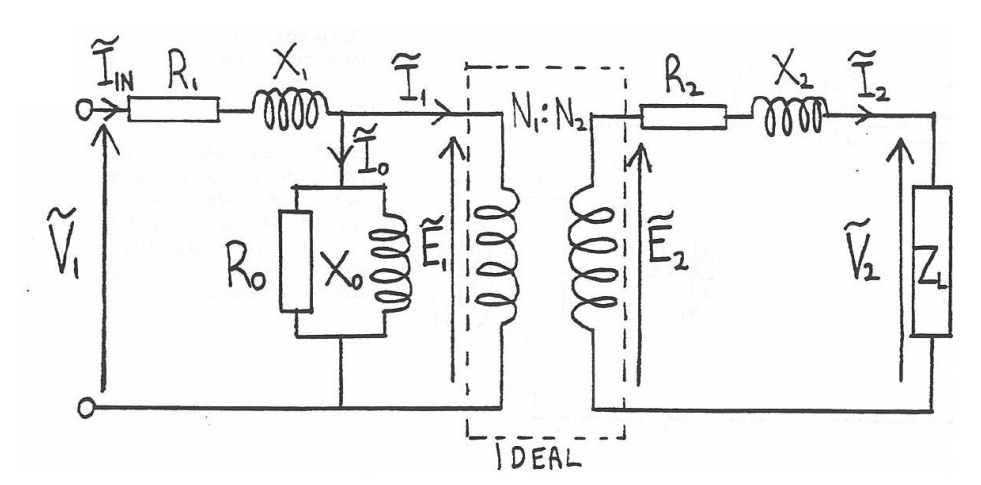
\includegraphics[width = 0.5\textwidth]{images/Screenshot 2024-04-05 160059.png}
    \caption{Real transformer model}
    \label{fig:enter-label}
\end{figure}

This is how the real transformer model looks like. There are further simplifications which can be done, for instance:

\begin{enumerate}
    \item Refer all copper losses from the secondary to the primary
    \item Because the copper losses are much smaller than the iron losses, we can move the parallel grouping before the series grouping
    \item The load can also be referred to the primary
\end{enumerate}

This then allows us to obtain a model for a real transformer with parameters $R_0, X_0$ (the iron losses) and $R_t, X_t$ (the copper losses).

\begin{figure}[h]
    \centering
    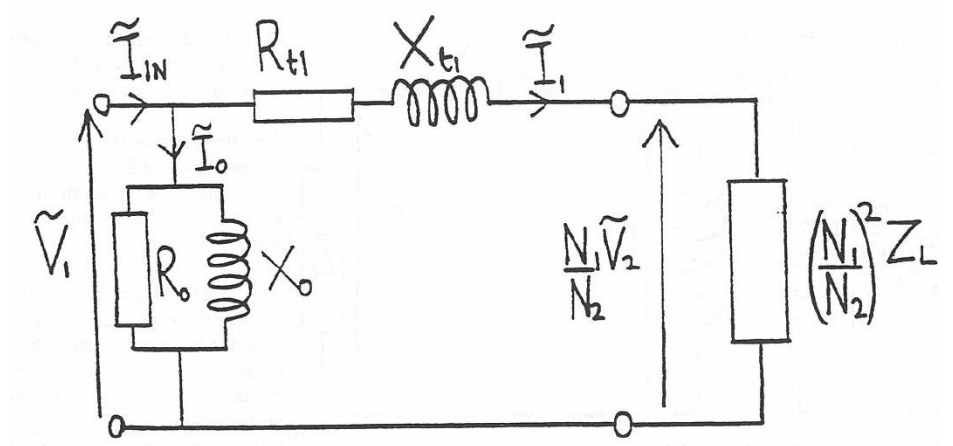
\includegraphics[width = 0.5\textwidth]{images/transf2.png}
    \caption{Real transformer, further simplifications}
    \label{fig:enter-label}
\end{figure}

To determine the various parameters of a transformer, we might use two tests. Note that these are also relevant for exam problems. The first one is called the open-circuit test, while the second one is the short-circuit test.

\subsubsection{The open-circuit test}

The primary of the transformer is excited, while the secondary remains open-circuited.

\begin{figure}[h]
    \centering
    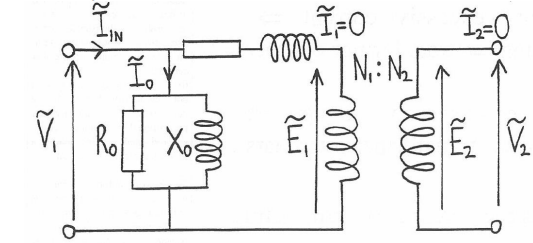
\includegraphics[width = 0.5\textwidth]{images/opencircuit.png}
    \caption{The open-circuit test}
    \label{fig:enter-label}
\end{figure}

Because the secondary is open-circuited, then $I_2 = 0$, and thus $I_1 = 0$. This means that effectively, the copper losses (series grouping) can be fully neglected (no current passing through). We can now just refer the two voltages, since:

\[ V_1 = E_1 \iff V_2 = E_2 \]

Furthermore:

\[ \frac{V_1}{V_2} = \frac{E_1}{E_2} = \frac{N_1}{N_2} \]

We also know that real power is consumed by the resistor only, so $P = \frac{V_1^2}{R_0}$, and reactive power is consumed by the magnetising reactance only, so $Q = \frac{V_1^2}{X_0}$. Using these facts, and whatever else we might get in the problem, we can deduce the values of $R_0$ and $X_0$ (the iron losses).

\subsubsection{The short-circuit test}

In the short-circuit test, the primary is excited, while the secondary remains short-circuited. 

\begin{figure}[h]
    \centering
    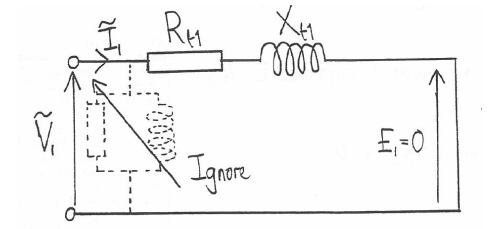
\includegraphics[width = 0.5\textwidth]{images/short.png}
    \caption{The short-circuit test}
    \label{fig:enter-label}
\end{figure}

Because of this, we have no voltage in the primary or secondary windings. Furthermore, we can fully ignore the parallel grouping. If the problem gives us details about the power consumed, then we can simply use:

\[ P = I_1^2R_t \iff Q = I_1^2X_t \]

To deduce the values of the copper losses.

\begin{definition}[Regulation]
    The regulation of a transformer is defined as the change in load voltage from the open-circuit value due to the load current. It is defined as:

    \[ r = \frac{V_{2_\text{oc}} - V_2}{V_{2_\text{oc}}} \] 
\end{definition}

\newpage

\section{Electromagnetics}

This chapter is a continuation of the first section of this course, in which we cover a few more aspects of electrostatics and electromagnetics. A majority of what was presented in the first handout is skipped, due to it already being presented at the beginning of this document.

\subsection{Electrostatics}

\begin{proposition}[Capacitance of air-filled coaxial cable]
    Consider an air-filled, cylindrical coaxial cable, filled with an inner conductor of diameter $2a$ and an outer conductor of diameter $2b$. Then, the capacitance per unit length of the cable is:

    \[ C_l = \frac{2\pi\epsilon_0}{\ln{\frac{b}{a}}} \] 
\end{proposition}

\begin{proof}
    Gauss' law states that:

    \[ \oiint_S \mathbf{D}\cdot d\mathbf{A} = Q \]

    Since we have a cylinder, i.e., a line of charge, then:

    \[ D \times 2\pi rL = \rho L \iff D \times 2\pi r = \rho \iff D = \frac{\rho}{2\pi r} \]

    Therefore, the electric field is:

    \[ E = \frac{\rho}{2\pi\epsilon_0 r} \]

    Now, we can use the Maxwell-Faraday law:

    \[ dV = -\mathbf{E} \cdot \mathbf{dl} \] 

    Therefore:

    \[ 0 - V = -\int_a^b \frac{\rho}{2\pi\epsilon_0 r}dr \iff V = \frac{\rho}{2\pi\epsilon_0}\ln{\frac{b}{a}} \]
    
    By definition, we have that $Q = CV \iff C = \frac{Q}{V}$. Therefore:

    \[ C = \frac{\rho L \times 2\pi\epsilon_0}{\rho \ln{\frac{b}{a}}} \]

    By dividing by $L$ to obtain the capacitance per unit length and simplifying:

    \[ C_l = \frac{2\pi\epsilon_0}{\ln{\frac{b}{a}}} \]
\end{proof}

Note that in the example above, if we had multiple substrates of dielectrics, we would have to integrate the electric fields between the respective ranges of each dielectric, obtaining a sum.

\begin{proposition}[Capacitance between two parallel wires]
    Consider two parallel cylindrical coaxial cables with their centres separated by a distance $2d$, and internal diameters of $2a$. Then, the capacitance per unit length between the two wires is:

    \[ C_l = \frac{\pi\epsilon_0}{\ln{\frac{2d - a}{a}}} \]
\end{proposition}

\begin{proof}
    The idea of this problem is to superpose the two electric flux densities/electric fields. As previously:

    \[ D = \frac{\rho}{2\pi r} \iff E = \frac{\rho}{2\pi\epsilon_0 r} \]

    If we now consider a coordinate system centred in between the two cylinders (in the middle of the line joining their centres), then, at position $x$ away from that point, the total electric field generated by both wires can be obtained by linear superposition:

    \[ E(x) = \frac{\rho}{2\pi\epsilon_0(d+x)} + \frac{\rho}{2\pi\epsilon_0(d - x)} \]

    Now, by Maxwell-Faraday:

    \[ V = \int_{-d + a}^{d - a} \left(\frac{\rho}{2\pi\epsilon_0(d+x)} + \frac{\rho}{2\pi\epsilon_0(d - x)}\right)dx \]
    \[ \iff V = \frac{\rho}{2\pi\epsilon_0}\int_{-d + a}^{d - a}\left(\frac{1}{d+x} + \frac{1}{d-x}\right)dx \]

    Which, by means of integration yields:

    \[ V = \frac{\rho}{\pi \epsilon_0}\ln{\frac{2d - a}{a}} \]

    By using $Q = CV$ as previously, we arrive to the conclusion.
\end{proof}

\subsubsection{Equipotentials and the method of images}

\begin{definition}[Equipotential]
    An equipotential is a line (or a surface) of constant potential. Equipotentials are lines along which we could move a point charge without having to do any work against electric fields.
\end{definition}

\begin{theorem}[The method of images]
    The method of images makes use of equipotentials. Consider the problem of calculating the electric field and potential of a point charge $Q$ at a height $h$ above a metal conducting plane. Because it is a conductor, the metal plane is an equipotential, and thus can be replcaed by an identical point charge at a distance $2h$ from the top one.
\end{theorem}

\begin{proof}
    We consider a coordinate system on the equipotential line at the middle between the two charges. We know that:

    \[ D = \frac{Q}{4\pi r^2} \]

    Then, by linear superposition:

    \[ E(x) = \frac{Q}{4\pi\epsilon_0}\left(\frac{1}{(h-x)^2} + \frac{1}{(h+x)^2}\right) \]
\end{proof}

\begin{figure}[h]
    \centering
    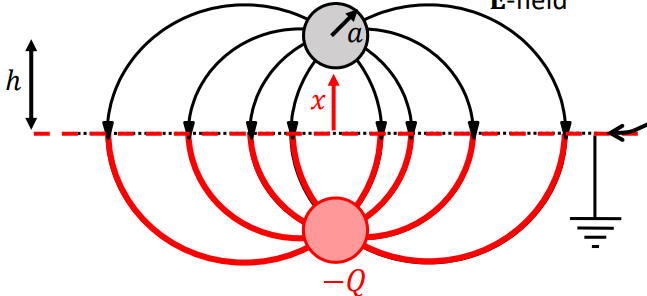
\includegraphics[width = 0.5\textwidth]{images/images.png}
    \caption{The method of images}
    \label{fig:enter-label}
\end{figure}

Note that this can then be further integrated from $0$ to $h - a$ to obtain the resulting voltage, and calculating the capacitance.

\subsubsection{Electrostatic energy}

\begin{proposition}[Energy of a capacitor]
    The energy stored in a capacitor of capacitance $C$, charge with a voltage $V$ is equal to:

    \[ E = \frac{1}{2}CV^2 \]
\end{proposition}

\begin{proof}
    The current is $I = \frac{\delta q}{\delta t}$. The voltage is $V = \frac{q}{C}$. The power is then:

    \[ P = VI = \frac{q}{C}\frac{\delta q}{\delta t} \]

    But $\delta W = P\delta t$, and hence:

    \[ \delta W = \frac{q}{C}\delta q\]

    By means of integration:

    \[ W = \int \frac{q}{C}dq = \frac{q^2}{2C} = \frac{CV^2}{2} \]
\end{proof}

\begin{proposition}[Electrostatic force]
    The force between the plates of a parallel-plate capacitor is:

    \[ F = \frac{1}{2}V^2\frac{\partial C}{\partial x} \]
\end{proposition}

\begin{proof}
    We use the principle of virtual work. The force $F$ does mechanical work against the "battery", equal to $-F \delta x$. The battery does work $V \delta q$ by providing the charge $\delta q$ in trying to keep the potential between the two conductors at a constant potential $V$. Also, there is a net change in electrostatic energy of:

    \[ dE = d\left(\frac{QV}{2}\right) = \frac{1}{2}Vdq \iff \delta E = \frac{1}{2}V \delta q \]

    Therefore:

    \[ -F \delta x + V \delta q = \frac{1}{2}V \delta q \]

    Hence:

    \[ -F\delta x = -\frac{1}{2}V\delta q \iff F = \frac{1}{2}V \frac{\delta q}{\delta x} \]

    Because we keep the potential constant, that means that $\delta q = V\delta C$, and therefore:

    \[ F = \frac{1}{2}V^2\frac{\delta C}{\delta x} \]

    In the limit where these changes are infinitesimally small:

    \[ F = \frac{1}{2}V^2\frac{\partial C}{\partial x} \]
\end{proof}

Note that this can then be used in problems. For a parallel plate capacitor, we know that:

\[ C = \frac{\epsilon S}{d} \]

If we add a depth parameter to this function:

\[ C(x) = \frac{\epsilon S}{x} \iff \frac{\partial C}{\partial x} = - \frac{\epsilon S}{x^2} \]

\subsection{Electromagnetics}

\begin{proposition}[Self inductance of a coaxial cable]
    Consider a cylindrical coaxial cable made of an inner conductor of diameter $2a$ and outer conductor of diameter $2b$. Therefore, the self inductance of this cable is given by:

    \[ L_l = \frac{\mu_0}{2\pi}\ln{\frac{b}{a}} \]
\end{proposition}

\begin{proof}
    By Ampere's law, we have that:

    \[ B \times 2\pi r = \mu_0 I \iff B = \frac{\mu_0 I}{2\pi r} \]

    The flux is given by:

    \[ \phi = \int_a^b \frac{\mu_0 I}{2\pi r}ldr = \frac{\mu_0 lI}{2\pi}\ln{\frac{b}{a}} \]

    The self inductance is $L = \frac{\phi}{I}$, and by accounting for the fact that we are interested in the inductance per unit length, it is trivial to now deduce the formula above.
\end{proof}

\subsubsection{Mutual inductance}

When two electrical circuits are close to one another, a current $I_1$ in the first one may cause a magnetic flux $\phi_2$ to link the other, and vice versa. Hence:

\[ \phi_2 = M_{12}I_1 \iff \phi_1 = M_{21}I_2 \]

The constants $M_{12}$ and $M_{21}$ are the mutual inductances of the circuit, and it is true that $M_{12} = M_{21} = M$, but the derivation of this is beyond the scope of this course.

\begin{example}[Mutual inductance of concentric solenoids]
    Consider a pair of concentric coils, the outer having $N_1$ turns per unit length, and the inner $N_2$ turns per unit length, cross sectional area $A$ and length $l$. The outer coil has a current $I$ passing through it, generating a magnetic flux $B$ along its axis. Therefore:

    \[ B = \mu_0N_1l \]

    The inner coil flux is $\phi_2 = BA$, and therefore the linked flux is:

    \[ \phi_2' = N_2lBA = N_2l(\mu_0N_1l)A \]

    The mutual inductance is $M = \frac{\phi_2'}{l}$. Therefore:

    \[ M = \mu_0N_1N_2lA \]
\end{example}

\begin{proposition}[Magnetic energy in current-carrying circuits]
    The magnetic energy stored in two self and mutually inducing coils is:

    \[ E = \frac{1}{2}L_1I_1^2 + \frac{1}{2}L_2I_2^2 + MI_1I_2 \]
\end{proposition}

\begin{proof}
    The flux linking the first coil is:

    \[ \phi_1 = L_1I_1 + MI_2 \]

    The flux linking the second coil is:

    \[ \phi_2 = L_2I_2 + MI_1 \]

    Therefore, since $V = \frac{d\phi}{dt}$, then $V_1 = L_1\frac{dI_1}{dt} + M\frac{dI_2}{dt}$, and $V_2 = L_2\frac{dI_2}{dt} + M\frac{dI_1}{dt}$. Now, using the fact that $P = \frac{dW}{dt} = I_1V_1 + I_2V_2$, one can easily deduce the proposition above.
\end{proof}

Note that the principles of energy conservation of virtual work can be applied to this expression, like we previously did for the electrostatics case, obtaining:

\[ F = I_1I_2\frac{\partial M}{\partial x} \]

However, this expression is not of much use, as it is pretty hard to obtain an analytical expression for $M = M(x)$.

\newpage

\subsubsection{Linear magnetic materials}

\begin{definition}[The magnetic field intensity]
    The magnetic field intensity $\mathbf{H}$ is defined so that its circulation around a closed loop equals the total current linking the loop. i.e.:

    \[ \oint_\Gamma \mathbf{H} \cdot \mathbf{dl} = NI \]
\end{definition}

\begin{proposition}[Magnetic flux density/intensity equivalence]
    For a linear magnetic material it is true that:

    \[ \mathbf{B} = \mu_0\mu_r\mathbf{H} \]
\end{proposition}

\begin{theorem}[Conservation of magnetic flux]
    Suppose we have a region $\Omega$ of space such that the magnetic flux density $\mathbf{B}$ lines are converging/contained/confined. Then, the total flux across the two areas will be the same.
\end{theorem}

\begin{example}[Magnetic flux in a toroidal electromagnet]
    For a toroidal electromagnet, we can simply apply Ampere's law:

    \[ Hl = NI \iff H \frac{NI}{l} \iff B = \frac{\mu_0\mu_r NI}{l} \]
\end{example}

\begin{example}[Magnetic flux in a toroidal electromagnet with an air gap]
    In this case, we have to be more careful when applying Ampere's law. We have to separate regions:

    \[ H_ml_m + H_gl_g = NI \iff \frac{B_m l_m}{\mu_0\mu_r} + \frac{B_g l_g}{\mu_0} = NI \]

    Note that flux is conserved, and since areas are equal, $B_m = B_g$. By rearranging the equation, we can obtain an expression for $B_m$ or $B_g$, since they are both equal.
\end{example}

\begin{example}[Magnetic flux in a non-linear electromagnet]
    We return to the above problem, but this time we assume that the material is no longer linear. Therefore:

    \[ H_m l_m + H_g l_g = NI \iff H_m l_m + \frac{B_g l_g}{\mu_0} = NI \]

    Note that we have not substituted the expression for $H_m$. Flux is conserved, so $B_m = B_g$. Therefore:

    \[ H_m l_m + \frac{B_m l_g}{\mu_0} = NI \]

    Therefore:

    \[ B_m = \frac{\mu_0(NI - H_m l_m)}{l_g} \]

    By intersecting this line (as a function of $H_m$) with the $B-H$ hysteresis curve, we can obtain the operating point of the electromagnet.
\end{example}

Note that if our problem gives us a permanent magnet, then we must set that $NI = 0$, since it produces magnetic flux without any current passing through it. A permanent magnet can be obtained through hysteresis by magnetising and de-magnetising a material.

\subsubsection{Magnetostatic energy}

\end{document}
